\documentclass[]{book}
\usepackage{lmodern}
\usepackage{amssymb,amsmath}
\usepackage{ifxetex,ifluatex}
\usepackage{fixltx2e} % provides \textsubscript
\ifnum 0\ifxetex 1\fi\ifluatex 1\fi=0 % if pdftex
  \usepackage[T1]{fontenc}
  \usepackage[utf8]{inputenc}
\else % if luatex or xelatex
  \ifxetex
    \usepackage{mathspec}
  \else
    \usepackage{fontspec}
  \fi
  \defaultfontfeatures{Ligatures=TeX,Scale=MatchLowercase}
\fi
% use upquote if available, for straight quotes in verbatim environments
\IfFileExists{upquote.sty}{\usepackage{upquote}}{}
% use microtype if available
\IfFileExists{microtype.sty}{%
\usepackage{microtype}
\UseMicrotypeSet[protrusion]{basicmath} % disable protrusion for tt fonts
}{}
\usepackage{hyperref}
\hypersetup{unicode=true,
            pdftitle={Multiple and Logistic Regression},
            pdfauthor={Your Name Here},
            pdfborder={0 0 0},
            breaklinks=true}
\urlstyle{same}  % don't use monospace font for urls
\usepackage{natbib}
\bibliographystyle{apalike}
\usepackage{color}
\usepackage{fancyvrb}
\newcommand{\VerbBar}{|}
\newcommand{\VERB}{\Verb[commandchars=\\\{\}]}
\DefineVerbatimEnvironment{Highlighting}{Verbatim}{commandchars=\\\{\}}
% Add ',fontsize=\small' for more characters per line
\usepackage{framed}
\definecolor{shadecolor}{RGB}{248,248,248}
\newenvironment{Shaded}{\begin{snugshade}}{\end{snugshade}}
\newcommand{\KeywordTok}[1]{\textcolor[rgb]{0.13,0.29,0.53}{\textbf{#1}}}
\newcommand{\DataTypeTok}[1]{\textcolor[rgb]{0.13,0.29,0.53}{#1}}
\newcommand{\DecValTok}[1]{\textcolor[rgb]{0.00,0.00,0.81}{#1}}
\newcommand{\BaseNTok}[1]{\textcolor[rgb]{0.00,0.00,0.81}{#1}}
\newcommand{\FloatTok}[1]{\textcolor[rgb]{0.00,0.00,0.81}{#1}}
\newcommand{\ConstantTok}[1]{\textcolor[rgb]{0.00,0.00,0.00}{#1}}
\newcommand{\CharTok}[1]{\textcolor[rgb]{0.31,0.60,0.02}{#1}}
\newcommand{\SpecialCharTok}[1]{\textcolor[rgb]{0.00,0.00,0.00}{#1}}
\newcommand{\StringTok}[1]{\textcolor[rgb]{0.31,0.60,0.02}{#1}}
\newcommand{\VerbatimStringTok}[1]{\textcolor[rgb]{0.31,0.60,0.02}{#1}}
\newcommand{\SpecialStringTok}[1]{\textcolor[rgb]{0.31,0.60,0.02}{#1}}
\newcommand{\ImportTok}[1]{#1}
\newcommand{\CommentTok}[1]{\textcolor[rgb]{0.56,0.35,0.01}{\textit{#1}}}
\newcommand{\DocumentationTok}[1]{\textcolor[rgb]{0.56,0.35,0.01}{\textbf{\textit{#1}}}}
\newcommand{\AnnotationTok}[1]{\textcolor[rgb]{0.56,0.35,0.01}{\textbf{\textit{#1}}}}
\newcommand{\CommentVarTok}[1]{\textcolor[rgb]{0.56,0.35,0.01}{\textbf{\textit{#1}}}}
\newcommand{\OtherTok}[1]{\textcolor[rgb]{0.56,0.35,0.01}{#1}}
\newcommand{\FunctionTok}[1]{\textcolor[rgb]{0.00,0.00,0.00}{#1}}
\newcommand{\VariableTok}[1]{\textcolor[rgb]{0.00,0.00,0.00}{#1}}
\newcommand{\ControlFlowTok}[1]{\textcolor[rgb]{0.13,0.29,0.53}{\textbf{#1}}}
\newcommand{\OperatorTok}[1]{\textcolor[rgb]{0.81,0.36,0.00}{\textbf{#1}}}
\newcommand{\BuiltInTok}[1]{#1}
\newcommand{\ExtensionTok}[1]{#1}
\newcommand{\PreprocessorTok}[1]{\textcolor[rgb]{0.56,0.35,0.01}{\textit{#1}}}
\newcommand{\AttributeTok}[1]{\textcolor[rgb]{0.77,0.63,0.00}{#1}}
\newcommand{\RegionMarkerTok}[1]{#1}
\newcommand{\InformationTok}[1]{\textcolor[rgb]{0.56,0.35,0.01}{\textbf{\textit{#1}}}}
\newcommand{\WarningTok}[1]{\textcolor[rgb]{0.56,0.35,0.01}{\textbf{\textit{#1}}}}
\newcommand{\AlertTok}[1]{\textcolor[rgb]{0.94,0.16,0.16}{#1}}
\newcommand{\ErrorTok}[1]{\textcolor[rgb]{0.64,0.00,0.00}{\textbf{#1}}}
\newcommand{\NormalTok}[1]{#1}
\usepackage{longtable,booktabs}
\usepackage{graphicx,grffile}
\makeatletter
\def\maxwidth{\ifdim\Gin@nat@width>\linewidth\linewidth\else\Gin@nat@width\fi}
\def\maxheight{\ifdim\Gin@nat@height>\textheight\textheight\else\Gin@nat@height\fi}
\makeatother
% Scale images if necessary, so that they will not overflow the page
% margins by default, and it is still possible to overwrite the defaults
% using explicit options in \includegraphics[width, height, ...]{}
\setkeys{Gin}{width=\maxwidth,height=\maxheight,keepaspectratio}
\IfFileExists{parskip.sty}{%
\usepackage{parskip}
}{% else
\setlength{\parindent}{0pt}
\setlength{\parskip}{6pt plus 2pt minus 1pt}
}
\setlength{\emergencystretch}{3em}  % prevent overfull lines
\providecommand{\tightlist}{%
  \setlength{\itemsep}{0pt}\setlength{\parskip}{0pt}}
\setcounter{secnumdepth}{5}
% Redefines (sub)paragraphs to behave more like sections
\ifx\paragraph\undefined\else
\let\oldparagraph\paragraph
\renewcommand{\paragraph}[1]{\oldparagraph{#1}\mbox{}}
\fi
\ifx\subparagraph\undefined\else
\let\oldsubparagraph\subparagraph
\renewcommand{\subparagraph}[1]{\oldsubparagraph{#1}\mbox{}}
\fi

%%% Use protect on footnotes to avoid problems with footnotes in titles
\let\rmarkdownfootnote\footnote%
\def\footnote{\protect\rmarkdownfootnote}

%%% Change title format to be more compact
\usepackage{titling}

% Create subtitle command for use in maketitle
\providecommand{\subtitle}[1]{
  \posttitle{
    \begin{center}\large#1\end{center}
    }
}

\setlength{\droptitle}{-2em}

  \title{\href{https://www.datacamp.com/courses/multiple-and-logistic-regression}{Multiple
and Logistic Regression}}
    \pretitle{\vspace{\droptitle}\centering\huge}
  \posttitle{\par}
    \author{\href{https://your_username.github.io/}{Your Name Here}}
    \preauthor{\centering\large\emph}
  \postauthor{\par}
      \predate{\centering\large\emph}
  \postdate{\par}
    \date{Last compiled: Oct 02, 2019}

\usepackage{booktabs}

\begin{document}
\maketitle

{
\setcounter{tocdepth}{1}
\tableofcontents
}
\chapter{Prerequisites}\label{prerequisites}

This material is from the \href{https://www.datacamp.com}{DataCamp}
course
\href{https://www.datacamp.com/courses/multiple-and-logistic-regression}{Multiple
and Logistic Regression} by Ben Baumer. Before using this material, the
reader should have completed and be comfortable with the material in the
DataCamp module
\href{https://www.datacamp.com/courses/correlation-and-regression}{Correlation
and Regression}.

Reminder to self: each \texttt{*.Rmd} file contains one and only one
chapter, and a chapter is defined by the first-level heading
\texttt{\#}.

\chapter{Parallel Slopes}\label{parallel-slopes}

In this chapter you'll learn about the class of linear models called
``parallel slopes models.'' These include one numeric and one
categorical explanatory variable.

\section{Fitting a parallel slopes
model}\label{fitting-a-parallel-slopes-model}

We use the \texttt{lm()} function to fit linear models to data. In this
case, we want to understand how the price of MarioKart games sold at
auction varies as a function of not only the number of wheels included
in the package, but also whether the item is new or used. Obviously, it
is expected that you might have to pay a premium to buy these new. But
how much is that premium? Can we estimate its value after
\emph{controlling for the number of wheels}?

We will fit a parallel slopes model using \texttt{lm()}. In addition to
the \texttt{data} argument, \texttt{lm()} needs to know which variables
you want to include in your regression model, and how you want to
include them. It accomplishes this using a \texttt{formula} argument. A
simple linear regression formula looks like
\texttt{y\ \textasciitilde{}\ x}, where \texttt{y} is the name of the
response variable, and \texttt{x} is the name of the explanatory
variable. Here, we will simply extend this formula to include multiple
explanatory variables. A parallel slopes model has the form
\texttt{y\ \textasciitilde{}\ x\ +\ z}, where \texttt{z} is a
categorical explanatory variable, and \texttt{x} is a numerical
explanatory variable.

The output from \texttt{lm()} is a model object, which when printed,
will show the fitted coefficients.

\begin{center}\rule{0.5\linewidth}{\linethickness}\end{center}

\subsection*{Exercise}\label{exercise}
\addcontentsline{toc}{subsection}{Exercise}

\begin{itemize}
\tightlist
\item
  The dataset \texttt{marioKart} is already loaded for you. Explore the
  data using \texttt{glimpse()} or \texttt{str()}.
\end{itemize}

\begin{Shaded}
\begin{Highlighting}[]
\KeywordTok{library}\NormalTok{(openintro)}
\KeywordTok{data}\NormalTok{(marioKart)}
\KeywordTok{glimpse}\NormalTok{(marioKart)}
\end{Highlighting}
\end{Shaded}

\begin{verbatim}
Observations: 143
Variables: 12
$ ID         <dbl> 150377422259, 260483376854, 320432342985, 280405224...
$ duration   <int> 3, 7, 3, 3, 1, 3, 1, 1, 3, 7, 1, 1, 1, 1, 7, 7, 3, ...
$ nBids      <int> 20, 13, 16, 18, 20, 19, 13, 15, 29, 8, 15, 15, 13, ...
$ cond       <fct> new, used, new, new, new, new, used, new, used, use...
$ startPr    <dbl> 0.99, 0.99, 0.99, 0.99, 0.01, 0.99, 0.01, 1.00, 0.9...
$ shipPr     <dbl> 4.00, 3.99, 3.50, 0.00, 0.00, 4.00, 0.00, 2.99, 4.0...
$ totalPr    <dbl> 51.55, 37.04, 45.50, 44.00, 71.00, 45.00, 37.02, 53...
$ shipSp     <fct> standard, firstClass, firstClass, standard, media, ...
$ sellerRate <int> 1580, 365, 998, 7, 820, 270144, 7284, 4858, 27, 201...
$ stockPhoto <fct> yes, yes, no, yes, yes, yes, yes, yes, yes, no, yes...
$ wheels     <int> 1, 1, 1, 1, 2, 0, 0, 2, 1, 1, 2, 2, 2, 2, 1, 0, 1, ...
$ title      <fct> "~~ Wii MARIO KART &amp; WHEEL ~ NINTENDO Wii ~ BRA...
\end{verbatim}

\begin{Shaded}
\begin{Highlighting}[]
\CommentTok{# Or}
\CommentTok{# str(marioKart)}
\CommentTok{# Data munging to agree with DataCamp mario_kart}
\NormalTok{mario_kart <-}\StringTok{ }\NormalTok{marioKart }\OperatorTok\StringTok{ }
\StringTok{  }\KeywordTok{filter}\NormalTok{(totalPr }\OperatorTok{<}\StringTok{ }\DecValTok{100}\NormalTok{)}
\KeywordTok{str}\NormalTok{(mario_kart)}
\end{Highlighting}
\end{Shaded}

\begin{verbatim}
'data.frame':   141 obs. of  12 variables:
 $ ID        : num  1.5e+11 2.6e+11 3.2e+11 2.8e+11 1.7e+11 ...
 $ duration  : int  3 7 3 3 1 3 1 1 3 7 ...
 $ nBids     : int  20 13 16 18 20 19 13 15 29 8 ...
 $ cond      : Factor w/ 2 levels "new","used": 1 2 1 1 1 1 2 1 2 2 ...
 $ startPr   : num  0.99 0.99 0.99 0.99 0.01 ...
 $ shipPr    : num  4 3.99 3.5 0 0 4 0 2.99 4 4 ...
 $ totalPr   : num  51.5 37 45.5 44 71 ...
 $ shipSp    : Factor w/ 8 levels "firstClass","media",..: 6 1 1 6 2 6 6 8 5 1 ...
 $ sellerRate: int  1580 365 998 7 820 270144 7284 4858 27 201 ...
 $ stockPhoto: Factor w/ 2 levels "no","yes": 2 2 1 2 2 2 2 2 2 1 ...
 $ wheels    : int  1 1 1 1 2 0 0 2 1 1 ...
 $ title     : Factor w/ 80 levels " Mario Kart Wii with Wii Wheel for Wii (New)",..: 80 60 22 7 4 19 34 5 79 70 ...
\end{verbatim}

\begin{Shaded}
\begin{Highlighting}[]
\KeywordTok{save}\NormalTok{(mario_kart,}\DataTypeTok{file =} \StringTok{"./Data/mario_kart.RData"}\NormalTok{)}
\end{Highlighting}
\end{Shaded}

\begin{itemize}
\tightlist
\item
  Use \texttt{lm()} to fit a parallel slopes model for total price as a
  function of the number of wheels and the condition of the item. Use
  the argument \texttt{data} to specify the dataset you're using.
\end{itemize}

\begin{Shaded}
\begin{Highlighting}[]
\CommentTok{# fit parallel slopes}
\KeywordTok{lm}\NormalTok{(totalPr }\OperatorTok{~}\StringTok{ }\NormalTok{wheels }\OperatorTok{+}\StringTok{ }\NormalTok{cond, }\DataTypeTok{data =}\NormalTok{ mario_kart)}
\end{Highlighting}
\end{Shaded}

\begin{verbatim}

Call:
lm(formula = totalPr ~ wheels + cond, data = mario_kart)

Coefficients:
(Intercept)       wheels     condused  
     42.370        7.233       -5.585  
\end{verbatim}

\begin{center}\rule{0.5\linewidth}{\linethickness}\end{center}

\subsection*{Reasoning about two
intercepts}\label{reasoning-about-two-intercepts}
\addcontentsline{toc}{subsection}{Reasoning about two intercepts}

The \texttt{marioKart} data contains several other variables. The
\texttt{totalPr}, \texttt{startPr}, and \texttt{shipPr} variables are
numeric, while the \texttt{cond} and \texttt{stockPhoto} variables are
categorical.

Which formula will result in a parallel slopes model?

\begin{itemize}
\item
  \texttt{totalPr\ \textasciitilde{}\ startPr\ +\ shipPr}
\item
  \texttt{cond\ \textasciitilde{}\ startPr\ +\ stockPhoto}
\item
  \textbf{\texttt{totalPr\ \textasciitilde{}\ shipPr\ +\ stockPhoto}}
\item
  \texttt{totalPr\ \textasciitilde{}\ cond}
\end{itemize}

\begin{center}\rule{0.5\linewidth}{\linethickness}\end{center}

\section{\texorpdfstring{Using \texttt{geom\_line()} and
\texttt{augment()}}{Using geom\_line() and augment()}}\label{using-geom_line-and-augment}

Parallel slopes models are so-named because we can visualize these
models in the data space as not one line, but two parallel lines. To do
this, we'll draw two things:

\begin{itemize}
\item
  a scatterplot showing the data, with color separating the points into
  groups
\item
  a line for each value of the categorical variable
\end{itemize}

Our plotting strategy is to compute the fitted values, plot these, and
connect the points to form a line. The \texttt{augment()} function from
the \texttt{broom} package provides an easy way to add the fitted values
to our data frame, and the \texttt{geom\_line()} function can then use
that data frame to plot the points and connect them.

Note that this approach has the added benefit of automatically coloring
the lines appropriately to match the data.

You already know how to use \texttt{ggplot()} and \texttt{geom\_point()}
to make the scatterplot. The only twist is that now you'll pass your
\texttt{augment()}-ed model as the data argument in your
\texttt{ggplot()} call. When you add your \texttt{geom\_line()}, instead
of letting the \texttt{y} aesthetic inherit its values from the
\texttt{ggplot()} call, you can set it to the \texttt{.fitted} column of
the \texttt{augment()}-ed model. This has the advantage of automatically
coloring the lines for you.

\begin{center}\rule{0.5\linewidth}{\linethickness}\end{center}

\subsection*{Exercise}\label{exercise-1}
\addcontentsline{toc}{subsection}{Exercise}

The parallel slopes model \texttt{mod} relating total price to the
number of wheels and condition is already in your workspace.

\begin{Shaded}
\begin{Highlighting}[]
\NormalTok{mod <-}\StringTok{ }\KeywordTok{lm}\NormalTok{(}\DataTypeTok{formula =}\NormalTok{ totalPr }\OperatorTok{~}\StringTok{ }\NormalTok{wheels }\OperatorTok{+}\StringTok{ }\NormalTok{cond, }\DataTypeTok{data =}\NormalTok{ mario_kart)}
\end{Highlighting}
\end{Shaded}

\begin{itemize}
\tightlist
\item
  \texttt{augment()} the model \texttt{mod} and explore the returned
  data frame using \texttt{glimpse()}. Notice the new variables that
  have been created.
\end{itemize}

\begin{Shaded}
\begin{Highlighting}[]
\KeywordTok{library}\NormalTok{(broom)}
\NormalTok{augmented_mod <-}\StringTok{ }\KeywordTok{augment}\NormalTok{(mod)}
\KeywordTok{glimpse}\NormalTok{(augmented_mod)}
\end{Highlighting}
\end{Shaded}

\begin{verbatim}
Observations: 141
Variables: 10
$ totalPr    <dbl> 51.55, 37.04, 45.50, 44.00, 71.00, 45.00, 37.02, 53...
$ wheels     <int> 1, 1, 1, 1, 2, 0, 0, 2, 1, 1, 2, 2, 2, 2, 1, 0, 1, ...
$ cond       <fct> new, used, new, new, new, new, used, new, used, use...
$ .fitted    <dbl> 49.60260, 44.01777, 49.60260, 49.60260, 56.83544, 4...
$ .se.fit    <dbl> 0.7087865, 0.5465195, 0.7087865, 0.7087865, 0.67645...
$ .resid     <dbl> 1.9473995, -6.9777674, -4.1026005, -5.6026005, 14.1...
$ .hat       <dbl> 0.02103158, 0.01250410, 0.02103158, 0.02103158, 0.0...
$ .sigma     <dbl> 4.902339, 4.868399, 4.892414, 4.881308, 4.750591, 4...
$ .cooksd    <dbl> 1.161354e-03, 8.712334e-03, 5.154337e-03, 9.612441e...
$ .std.resid <dbl> 0.40270893, -1.43671086, -0.84838977, -1.15857953, ...
\end{verbatim}

\begin{itemize}
\tightlist
\item
  Draw the scatterplot and save it as \texttt{data\_space} by passing
  the \texttt{augment()}-ed model to \texttt{ggplot()} and using
  \texttt{geom\_point()}.
\end{itemize}

\begin{Shaded}
\begin{Highlighting}[]
\CommentTok{# scatterplot, with color}
\NormalTok{data_space <-}\StringTok{ }\KeywordTok{ggplot}\NormalTok{(}\DataTypeTok{data =}\NormalTok{ augmented_mod, }
                     \KeywordTok{aes}\NormalTok{(}\DataTypeTok{x =}\NormalTok{ wheels, }\DataTypeTok{y =}\NormalTok{ totalPr, }
                         \DataTypeTok{color =}\NormalTok{ cond)) }\OperatorTok{+}\StringTok{ }
\StringTok{  }\KeywordTok{geom_point}\NormalTok{()}
\end{Highlighting}
\end{Shaded}

\begin{itemize}
\tightlist
\item
  Use \texttt{geom\_line()} once to add two parallel lines corresponding
  to our model.
\end{itemize}

\begin{Shaded}
\begin{Highlighting}[]
\CommentTok{# single call to geom_line()}
\NormalTok{data_space }\OperatorTok{+}\StringTok{ }
\StringTok{  }\KeywordTok{geom_line}\NormalTok{(}\KeywordTok{aes}\NormalTok{(}\DataTypeTok{x =}\NormalTok{ wheels, }\DataTypeTok{y =}\NormalTok{ .fitted)) }\OperatorTok{+}\StringTok{ }
\StringTok{  }\KeywordTok{theme_bw}\NormalTok{()}
\end{Highlighting}
\end{Shaded}

\begin{center}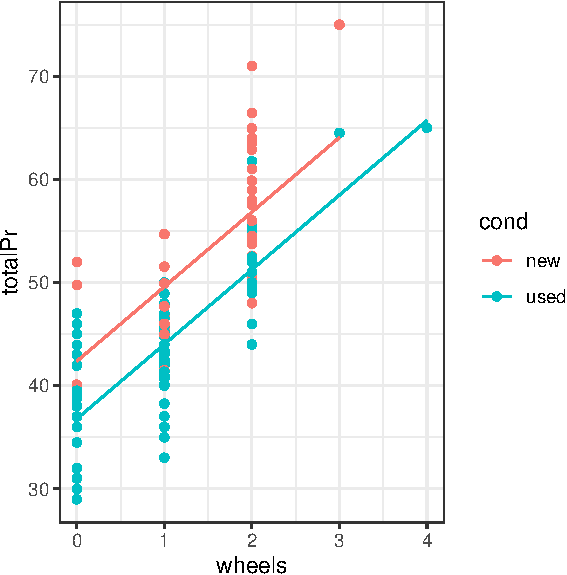
\includegraphics{MultLogSC_files/figure-latex/unnamed-chunk-7-1} \end{center}

\begin{center}\rule{0.5\linewidth}{\linethickness}\end{center}

\subsection*{Intercept interpretation}\label{intercept-interpretation}
\addcontentsline{toc}{subsection}{Intercept interpretation}

Recall that the \texttt{cond} variable is either \texttt{new} or
\texttt{used}. Here are the fitted coefficients from your model:

\begin{Shaded}
\begin{Highlighting}[]
\KeywordTok{lm}\NormalTok{(totalPr }\OperatorTok{~}\StringTok{ }\NormalTok{wheels }\OperatorTok{+}\StringTok{ }\NormalTok{cond, }\DataTypeTok{data =}\NormalTok{ mario_kart)}
\end{Highlighting}
\end{Shaded}

\begin{verbatim}

Call:
lm(formula = totalPr ~ wheels + cond, data = mario_kart)

Coefficients:
(Intercept)       wheels     condused  
     42.370        7.233       -5.585  
\end{verbatim}

Choose the correct interpretation of the coefficient on
\texttt{condused}:

\begin{itemize}
\item
  For each additional wheel, the expected price of a used MarioKart is
  \$5.58 lower.
\item
  \textbf{The expected price of a used MarioKart is \$5.58 less than
  that of a new one with the same number of wheels.}
\item
  The expected price of a new MarioKart is \$5.58 less than that of a
  used one with the same number of wheels.
\item
  The used MarioKarts are always \$5.58 cheaper.
\end{itemize}

\begin{center}\rule{0.5\linewidth}{\linethickness}\end{center}

\subsection*{Common slope
interpretation}\label{common-slope-interpretation}
\addcontentsline{toc}{subsection}{Common slope interpretation}

Recall the fitted coefficients from our model:

\begin{Shaded}
\begin{Highlighting}[]
\KeywordTok{lm}\NormalTok{(totalPr }\OperatorTok{~}\StringTok{ }\NormalTok{wheels }\OperatorTok{+}\StringTok{ }\NormalTok{cond, }\DataTypeTok{data =}\NormalTok{ mario_kart)}
\end{Highlighting}
\end{Shaded}

\begin{verbatim}

Call:
lm(formula = totalPr ~ wheels + cond, data = mario_kart)

Coefficients:
(Intercept)       wheels     condused  
     42.370        7.233       -5.585  
\end{verbatim}

Choose the correct interpretation of the slope coefficient:

\begin{itemize}
\item
  \textbf{For each additional wheel, the expected price of a MarioKart
  increases by \$7.23 regardless of whether it is new or used.}
\item
  For each additional wheel, the expected price of a new MarioKart
  increases by \$7.23.
\item
  The expected price of a used MarioKart is \$5.59 less than that of a
  new one with the same number of wheels.
\item
  You should always expect to pay \$42.37 for a MarioKart.
\end{itemize}

\begin{center}\rule{0.5\linewidth}{\linethickness}\end{center}

\section{Syntax from math}\label{syntax-from-math}

The \texttt{babies} data set contains observations about the birthweight
and other characteristics of children born in the San Francisco Bay area
from 1960--1967.

We would like to build a model for birthweight as a function of the
mother's age and whether this child was her first
(\texttt{parity\ ==\ 0}). Use the mathematical specification below to
code the model in R.

\[birthweight=\beta_0 + \beta_1 \cdot age + \beta_2 \cdot parity + \varepsilon\]

\begin{center}\rule{0.5\linewidth}{\linethickness}\end{center}

\subsection*{Exercise}\label{exercise-2}
\addcontentsline{toc}{subsection}{Exercise}

The birthweight variable is recorded in the column \texttt{bwt}.

\begin{itemize}
\tightlist
\item
  Use \texttt{lm()} to build the parallel slopes model specified above.
  It's not necessary to use \texttt{factor()} in this case as the
  variable \texttt{parity} is coded using binary numeric values.
\end{itemize}

\begin{Shaded}
\begin{Highlighting}[]
\CommentTok{# build model}
\KeywordTok{lm}\NormalTok{(bwt }\OperatorTok{~}\StringTok{ }\NormalTok{age }\OperatorTok{+}\StringTok{ }\NormalTok{parity, }\DataTypeTok{data =}\NormalTok{ babies)}
\end{Highlighting}
\end{Shaded}

\begin{verbatim}

Call:
lm(formula = bwt ~ age + parity, data = babies)

Coefficients:
(Intercept)          age       parity  
  118.27782      0.06315     -1.65248  
\end{verbatim}

\begin{center}\rule{0.5\linewidth}{\linethickness}\end{center}

\section{Syntax from plot}\label{syntax-from-plot}

This time, we'd like to build a model for birthweight as a function of
the length of gestation and the mother's smoking status. Use Figure
\ref{fig:SmokP1} to inform your model specification.

\begin{Shaded}
\begin{Highlighting}[]
\KeywordTok{ggplot}\NormalTok{(}\DataTypeTok{data =}\NormalTok{ babies, }\KeywordTok{aes}\NormalTok{(}\DataTypeTok{x =}\NormalTok{ gestation, }\DataTypeTok{y =}\NormalTok{ bwt, }\DataTypeTok{color =} \KeywordTok{factor}\NormalTok{(smoke))) }\OperatorTok{+}
\StringTok{  }\KeywordTok{geom_point}\NormalTok{(}\DataTypeTok{alpha =} \FloatTok{0.5}\NormalTok{) }\OperatorTok{+}
\StringTok{  }\KeywordTok{theme_bw}\NormalTok{()}
\end{Highlighting}
\end{Shaded}

\begin{figure}

{\centering 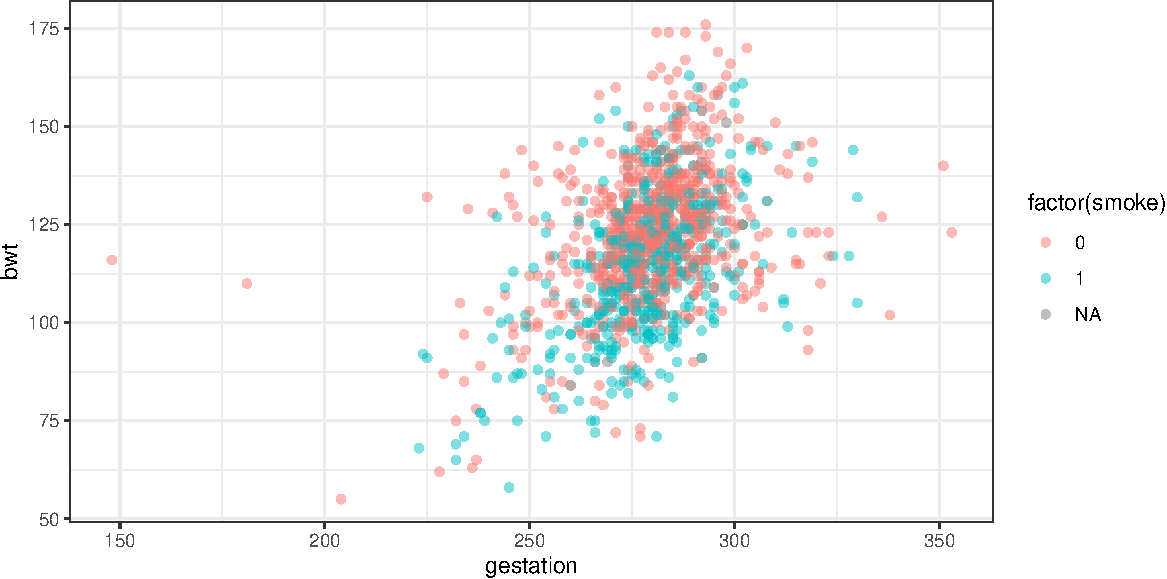
\includegraphics{MultLogSC_files/figure-latex/SmokP1-1} 

}

\caption{`bwt` versus `gestation`}\label{fig:SmokP1}
\end{figure}

\begin{center}\rule{0.5\linewidth}{\linethickness}\end{center}

\subsection*{Exercise}\label{exercise-3}
\addcontentsline{toc}{subsection}{Exercise}

\begin{itemize}
\tightlist
\item
  Use \texttt{lm()} to build a parallel slopes model implied by the
  plot. It's not necessary to use \texttt{factor()} in this case either.
\end{itemize}

\begin{Shaded}
\begin{Highlighting}[]
\CommentTok{# build model}
\KeywordTok{lm}\NormalTok{(bwt }\OperatorTok{~}\StringTok{ }\NormalTok{gestation }\OperatorTok{+}\StringTok{ }\NormalTok{smoke, }\DataTypeTok{data =}\NormalTok{ babies)}
\end{Highlighting}
\end{Shaded}

\begin{verbatim}

Call:
lm(formula = bwt ~ gestation + smoke, data = babies)

Coefficients:
(Intercept)    gestation        smoke  
    -0.9317       0.4429      -8.0883  
\end{verbatim}

\begin{center}\rule{0.5\linewidth}{\linethickness}\end{center}

\chapter{Evaluating and extending parallel slopes
model}\label{evaluating-and-extending-parallel-slopes-model}

This chapter covers model evaluation. By looking at different properties
of the model, including the adjusted R-squared, you'll learn to compare
models so that you can select the best one. You'll also learn about
interaction terms in linear models.

\section{R-squared vs.~adjusted
R-squared}\label{r-squared-vs.adjusted-r-squared}

Two common measures of how well a model fits to data are \(R^2\) (the
coefficient of determination) and the adjusted \(R^2\). The former
measures the percentage of the variability in the response variable that
is explained by the model. To compute this, we define

\[R^2 = 1 − \frac{SSE}{SST},\] where \(SSE\) and \(SST\) are the sum of
the squared residuals, and the total sum of the squares, respectively.
One issue with this measure is that the \(SSE\) can only decrease as new
variable are added to the model, while the \(SST\) depends only on the
response variable and therefore is not affected by changes to the model.
This means that you can increase \(R^2\) by adding any additional
variable to your model---even random noise.

The adjusted \(R^2\) includes a term that penalizes a model for each
additional explanatory variable (where \(p\) is the number of
explanatory variables).

\[R^2_{\text{adj}} = 1 − \frac{SSE}{SST}\cdot\frac{n-1}{n-p-1},\]

We can see both measures in the output of the \texttt{summary()}
function on our model object.

\begin{center}\rule{0.5\linewidth}{\linethickness}\end{center}

\subsection*{Exercise}\label{exercise-4}
\addcontentsline{toc}{subsection}{Exercise}

\begin{Shaded}
\begin{Highlighting}[]
\KeywordTok{load}\NormalTok{(}\StringTok{"./Data/mario_kart.RData"}\NormalTok{)}
\NormalTok{mod <-}\StringTok{ }\KeywordTok{lm}\NormalTok{(totalPr }\OperatorTok{~}\StringTok{ }\NormalTok{wheels }\OperatorTok{+}\StringTok{ }\NormalTok{cond, }\DataTypeTok{data =}\NormalTok{ mario_kart)}
\end{Highlighting}
\end{Shaded}

\begin{itemize}
\tightlist
\item
  Use \texttt{summary()} to compute \(R^2\) and adjusted \(R^2\) on the
  model object called \texttt{mod}.
\end{itemize}

\begin{Shaded}
\begin{Highlighting}[]
\CommentTok{# R^2 and adjusted R^2}
\KeywordTok{summary}\NormalTok{(mod)}
\end{Highlighting}
\end{Shaded}

\begin{verbatim}

Call:
lm(formula = totalPr ~ wheels + cond, data = mario_kart)

Residuals:
     Min       1Q   Median       3Q      Max 
-11.0078  -3.0754  -0.8254   2.9822  14.1646 

Coefficients:
            Estimate Std. Error t value Pr(>|t|)    
(Intercept)  42.3698     1.0651  39.780  < 2e-16 ***
wheels        7.2328     0.5419  13.347  < 2e-16 ***
condused     -5.5848     0.9245  -6.041 1.35e-08 ***
---
Signif. codes:  0 '***' 0.001 '**' 0.01 '*' 0.05 '.' 0.1 ' ' 1

Residual standard error: 4.887 on 138 degrees of freedom
Multiple R-squared:  0.7165,    Adjusted R-squared:  0.7124 
F-statistic: 174.4 on 2 and 138 DF,  p-value: < 2.2e-16
\end{verbatim}

The \(R^2\) value for \texttt{mod} is 0.7165182, and the
\(R^2_{\text{adj}}\) value is 0.7124098.

\begin{itemize}
\tightlist
\item
  Use \texttt{mutate()} and \texttt{rnorm()} to add a new variable
  called \texttt{noise} to the \texttt{mario\_kart} data set that
  consists of random noise. Save the new dataframe as
  \texttt{mario\_kart\_noisy}.
\end{itemize}

\begin{Shaded}
\begin{Highlighting}[]
\CommentTok{# add random noise}
\KeywordTok{set.seed}\NormalTok{(}\DecValTok{34}\NormalTok{)}
\CommentTok{# add random noise}
\NormalTok{mario_kart_noisy <-}\StringTok{ }\NormalTok{mario_kart }\OperatorTok
\StringTok{  }\KeywordTok{mutate}\NormalTok{(}\DataTypeTok{noise =} \KeywordTok{rnorm}\NormalTok{(}\KeywordTok{nrow}\NormalTok{(mario_kart)))}
\end{Highlighting}
\end{Shaded}

\begin{itemize}
\tightlist
\item
  Use \texttt{lm()} to fit a model that includes \texttt{wheels},
  \texttt{cond}, and the random noise term.
\end{itemize}

\begin{Shaded}
\begin{Highlighting}[]
\CommentTok{# compute new model}
\NormalTok{mod2 <-}\StringTok{ }\KeywordTok{lm}\NormalTok{(totalPr }\OperatorTok{~}\StringTok{ }\NormalTok{wheels }\OperatorTok{+}\StringTok{ }\NormalTok{cond }\OperatorTok{+}\StringTok{ }\NormalTok{noise, }\DataTypeTok{data =}\NormalTok{ mario_kart_noisy)}
\end{Highlighting}
\end{Shaded}

\begin{itemize}
\tightlist
\item
  Use \texttt{summary()} to compute \(R^2\) and adjusted \(R^2\) on the
  new model object. Did the value of \(R^2\) increase? \textbf{Yes} What
  about adjusted \(R^2\)? \textbf{It also increased.} \textbf{Adding
  random noise increase both \(R^2\) and \(R^2_{\text{adj}}\).}
\end{itemize}

\begin{Shaded}
\begin{Highlighting}[]
\CommentTok{# new R^2 and adjusted R^2}
\KeywordTok{summary}\NormalTok{(mod2)}
\end{Highlighting}
\end{Shaded}

\begin{verbatim}

Call:
lm(formula = totalPr ~ wheels + cond + noise, data = mario_kart_noisy)

Residuals:
     Min       1Q   Median       3Q      Max 
-10.3256  -3.1692  -0.7492   2.8731  14.1293 

Coefficients:
            Estimate Std. Error t value Pr(>|t|)    
(Intercept)  42.2788     1.0659  39.664  < 2e-16 ***
wheels        7.2310     0.5410  13.367  < 2e-16 ***
condused     -5.4003     0.9354  -5.774 4.97e-08 ***
noise        -0.4930     0.4059  -1.215    0.227    
---
Signif. codes:  0 '***' 0.001 '**' 0.01 '*' 0.05 '.' 0.1 ' ' 1

Residual standard error: 4.879 on 137 degrees of freedom
Multiple R-squared:  0.7195,    Adjusted R-squared:  0.7134 
F-statistic: 117.2 on 3 and 137 DF,  p-value: < 2.2e-16
\end{verbatim}

\begin{center}\rule{0.5\linewidth}{\linethickness}\end{center}

\section{Prediction}\label{prediction}

Once we have fit a regression model, we can use it to make predictions
for unseen observations or retrieve the fitted values. Here, we explore
two methods for doing the latter.

A traditional way to return the fitted values (i.e.~the \(\hat{y}\)'s)
is to run the \texttt{predict()} function on the model object. This will
return a vector of the fitted values. Note that \texttt{predict()} will
take an optional \texttt{newdata} argument that will allow you to make
predictions for observations that are not in the original data.

A newer alternative is the \texttt{augment()} function from the
\texttt{broom} package, which returns a \texttt{data.frame} with the
response variable (\(y\)), the relevant explanatory variables (the
\(x\)'s), the fitted value (\(\hat{y}\)) and some information about the
residuals (\(\hat{\varepsilon}\)). \texttt{augment()} will also take a
\texttt{newdata} argument that allows you to make predictions.

\begin{center}\rule{0.5\linewidth}{\linethickness}\end{center}

\subsection*{Exercise}\label{exercise-5}
\addcontentsline{toc}{subsection}{Exercise}

The fitted model \texttt{mod} is already in your environment.

\begin{itemize}
\tightlist
\item
  Compute the fitted values of the model as a vector using
  \texttt{predict()}.
\end{itemize}

\begin{Shaded}
\begin{Highlighting}[]
\CommentTok{# return a vector}
\NormalTok{VEC <-}\StringTok{ }\KeywordTok{predict}\NormalTok{(mod)}
\KeywordTok{head}\NormalTok{(VEC)}
\end{Highlighting}
\end{Shaded}

\begin{verbatim}
       1        2        3        4        5        6 
49.60260 44.01777 49.60260 49.60260 56.83544 42.36976 
\end{verbatim}

\begin{itemize}
\tightlist
\item
  Compute the fitted values of the model as one column in a
  \texttt{data.frame} using \texttt{augment()}.
\end{itemize}

\begin{Shaded}
\begin{Highlighting}[]
\CommentTok{# return a data frame}
\NormalTok{DF <-}\StringTok{ }\NormalTok{broom}\OperatorTok{::}\KeywordTok{augment}\NormalTok{(mod)}
\KeywordTok{head}\NormalTok{(DF)}
\end{Highlighting}
\end{Shaded}

\begin{verbatim}
# A tibble: 6 x 10
  totalPr wheels cond  .fitted .se.fit .resid   .hat .sigma .cooksd
    <dbl>  <int> <fct>   <dbl>   <dbl>  <dbl>  <dbl>  <dbl>   <dbl>
1    51.6      1 new      49.6   0.709   1.95 0.0210   4.90 0.00116
2    37.0      1 used     44.0   0.547  -6.98 0.0125   4.87 0.00871
3    45.5      1 new      49.6   0.709  -4.10 0.0210   4.89 0.00515
4    44        1 new      49.6   0.709  -5.60 0.0210   4.88 0.00961
5    71        2 new      56.8   0.676  14.2  0.0192   4.75 0.0557 
6    45        0 new      42.4   1.07    2.63 0.0475   4.90 0.00505
# ... with 1 more variable: .std.resid <dbl>
\end{verbatim}

\begin{center}\rule{0.5\linewidth}{\linethickness}\end{center}

\subsection*{Thought experiments}\label{thought-experiments}
\addcontentsline{toc}{subsection}{Thought experiments}

Suppose that after going apple picking you have 12 apples left over. You
decide to conduct an experiment to investigate how quickly they will rot
under certain conditions. You place six apples in a cool spot in your
basement, and leave the other six on the window sill in the kitchen.
Every week, you estimate the percentage of the surface area of the apple
that is rotten or moldy.

Consider the following models:

\[rot=\beta_0 + \beta_1\cdot t + \beta_2 \cdot temp,\]

and

\[rot=\beta_0 + \beta_1\cdot t + \beta_2 \cdot temp + \beta_3 \cdot temp \cdot t,\]

where \(t\) is time, measured in weeks, and \(temp\) is a binary
variable indicating either cool or warm.

If you decide to keep the interaction term present in the second model,
you are implicitly assuming that:

\begin{center}\rule{0.5\linewidth}{\linethickness}\end{center}

\begin{itemize}
\item
  The amount of rot will vary based on the temperature.
\item
  The amount of rot will vary based on the temperature, after
  controlling for the length of time they have been left out.
\item
  \textbf{The rate at which apples rot will vary based on the
  temperature.}
\item
  Time and temperature are independent.
\end{itemize}

\begin{center}\rule{0.5\linewidth}{\linethickness}\end{center}

\section{Fitting a model with
interaction}\label{fitting-a-model-with-interaction}

Including an interaction term in a model is easy---we just have to tell
\texttt{lm()} that we want to include that new variable. An expression
of the form

\begin{Shaded}
\begin{Highlighting}[]
\KeywordTok{lm}\NormalTok{(y }\OperatorTok{~}\StringTok{ }\NormalTok{x }\OperatorTok{+}\StringTok{ }\NormalTok{z }\OperatorTok{+}\StringTok{ }\NormalTok{x}\OperatorTok{:}\NormalTok{z, }\DataTypeTok{data =}\NormalTok{ mydata)}
\end{Highlighting}
\end{Shaded}

will do the trick. The use of the colon (\texttt{:}) here means that the
interaction between \texttt{x} and \texttt{z} will be a third term in
the model.

\begin{center}\rule{0.5\linewidth}{\linethickness}\end{center}

\subsection*{Exercise}\label{exercise-6}
\addcontentsline{toc}{subsection}{Exercise}

The data frame \texttt{mario\_kart} is already loaded in your workspace.

\begin{itemize}
\tightlist
\item
  Use \texttt{lm()} to fit a model for the price of a MarioKart as a
  function of its condition and the duration of the auction, with
  interaction.
\end{itemize}

\begin{Shaded}
\begin{Highlighting}[]
\CommentTok{# include interaction}
\KeywordTok{lm}\NormalTok{(totalPr }\OperatorTok{~}\StringTok{ }\NormalTok{cond }\OperatorTok{+}\StringTok{ }\NormalTok{duration }\OperatorTok{+}\StringTok{ }\NormalTok{cond}\OperatorTok{:}\NormalTok{duration, }\DataTypeTok{data =}\NormalTok{ mario_kart)}
\end{Highlighting}
\end{Shaded}

\begin{verbatim}

Call:
lm(formula = totalPr ~ cond + duration + cond:duration, data = mario_kart)

Coefficients:
      (Intercept)           condused           duration  
           58.268            -17.122             -1.966  
condused:duration  
            2.325  
\end{verbatim}

\begin{center}\rule{0.5\linewidth}{\linethickness}\end{center}

\section{Visualizing interaction
models}\label{visualizing-interaction-models}

Interaction allows the slope of the regression line in each group to
vary. In this case, this means that the relationship between the final
price and the length of the auction is moderated by the condition of
each item.

Interaction models are easy to visualize in the data space with
\texttt{ggplot2} because they have the same coefficients as if the
models were fit independently to each group defined by the level of the
categorical variable. In this case, new and used MarioKarts each get
their own regression line. To see this, we can set an aesthetic (e.g.
\texttt{color}) to the categorical variable, and then add a
\texttt{geom\_smooth()} layer to overlay the regression line for each
color.

\begin{center}\rule{0.5\linewidth}{\linethickness}\end{center}

\section*{Exercise}\label{exercise-7}
\addcontentsline{toc}{section}{Exercise}

The dataset \texttt{mario\_kart} is already loaded in your workspace.

\begin{itemize}
\tightlist
\item
  Use the \texttt{color} aesthetic and the \texttt{geom\_smooth()}
  function to plot the interaction model between duration and condition
  in the data space. Make sure you set the \texttt{method} and
  \texttt{se} arguments of \texttt{geom\_smooth()}.
\end{itemize}

\begin{Shaded}
\begin{Highlighting}[]
\CommentTok{# interaction plot}
\KeywordTok{ggplot}\NormalTok{(}\DataTypeTok{data =}\NormalTok{ mario_kart, }\KeywordTok{aes}\NormalTok{(}\DataTypeTok{y =}\NormalTok{ totalPr, }\DataTypeTok{x =}\NormalTok{ duration, }\DataTypeTok{color =}\NormalTok{ cond)) }\OperatorTok{+}
\StringTok{  }\KeywordTok{geom_point}\NormalTok{() }\OperatorTok{+}\StringTok{ }
\StringTok{  }\KeywordTok{geom_smooth}\NormalTok{(}\DataTypeTok{method =} \StringTok{"lm"}\NormalTok{, }\DataTypeTok{se =} \OtherTok{FALSE}\NormalTok{) }\OperatorTok{+}
\StringTok{  }\KeywordTok{theme_bw}\NormalTok{()}
\end{Highlighting}
\end{Shaded}

\begin{center}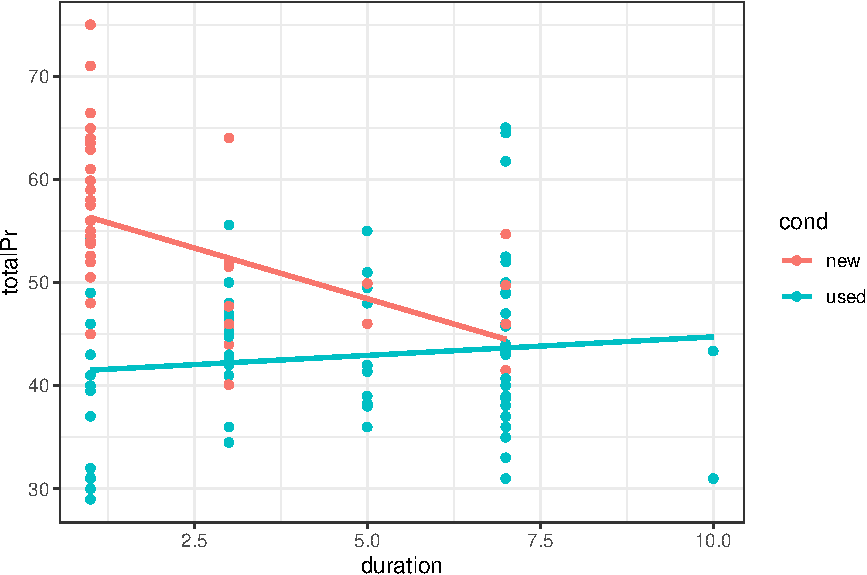
\includegraphics{MultLogSC_files/figure-latex/unnamed-chunk-21-1} \end{center}

\begin{itemize}
\tightlist
\item
  How does the interaction model differ from the parallel slopes model?
  \textbf{Class discussion}
\end{itemize}

\begin{center}\rule{0.5\linewidth}{\linethickness}\end{center}

\section{Consequences of Simpson's
paradox}\label{consequences-of-simpsons-paradox}

In the simple linear regression model for average SAT score,
(\texttt{total}) as a function of average teacher salary
(\texttt{salary}), the fitted coefficient was -5.02 points per thousand
dollars. This suggests that for every additional thousand dollars of
salary for teachers in a particular state, the expected SAT score for a
student from that state is about 5 points lower.

In the model that includes the percentage of students taking the SAT,
the coefficient on \texttt{salary} becomes 1.84 points per thousand
dollars. Choose the correct interpretation of this slope coefficient.

\begin{Shaded}
\begin{Highlighting}[]
\NormalTok{SAT <-}\StringTok{ }\KeywordTok{read.csv}\NormalTok{(}\StringTok{"https://assets.datacamp.com/production/repositories/845/datasets/1a12a19d2cec83ca0b58645689987e2025d91383/SAT.csv"}\NormalTok{)}
\KeywordTok{lm}\NormalTok{(total }\OperatorTok{~}\StringTok{ }\NormalTok{salary, }\DataTypeTok{data =}\NormalTok{ SAT)}
\end{Highlighting}
\end{Shaded}

\begin{verbatim}

Call:
lm(formula = total ~ salary, data = SAT)

Coefficients:
(Intercept)       salary  
  1.871e+03   -5.019e-03  
\end{verbatim}

\begin{Shaded}
\begin{Highlighting}[]
\NormalTok{SAT_wbin <-}\StringTok{ }\NormalTok{SAT }\OperatorTok
\StringTok{    }\KeywordTok{mutate}\NormalTok{(}\DataTypeTok{sat_bin =} \KeywordTok{cut}\NormalTok{(sat_pct, }\DecValTok{3}\NormalTok{))}
\NormalTok{mod <-}\StringTok{ }\KeywordTok{lm}\NormalTok{(}\DataTypeTok{formula =}\NormalTok{ total }\OperatorTok{~}\StringTok{ }\NormalTok{salary }\OperatorTok{+}\StringTok{ }\NormalTok{sat_bin, }\DataTypeTok{data =}\NormalTok{ SAT_wbin)}
\NormalTok{mod}
\end{Highlighting}
\end{Shaded}

\begin{verbatim}

Call:
lm(formula = total ~ salary + sat_bin, data = SAT_wbin)

Coefficients:
     (Intercept)            salary    sat_bin(33,63]  sat_bin(63,93.1]  
      1597.10773           0.00184        -191.45221        -217.73480  
\end{verbatim}

\begin{center}\rule{0.5\linewidth}{\linethickness}\end{center}

\begin{itemize}
\item
  For every additional thousand dollars of salary for teachers in a
  particular state, the expected SAT score for a student from that state
  is about 2 points lower.
\item
  \textbf{For every additional thousand dollars of salary for teachers
  in a particular state, the expected SAT score for a student from that
  state is about 2 points higher, after controlling for the percentage
  of students taking the SAT.}
\item
  The average SAT score in richer states is about 2 points higher.
\end{itemize}

\begin{center}\rule{0.5\linewidth}{\linethickness}\end{center}

\section{Simpson's paradox in action}\label{simpsons-paradox-in-action}

A mild version of
\href{https://en.wikipedia.org/wiki/Simpson\%27s_paradox}{Simpson's
paradox} can be observed in the MarioKart auction data. Consider the
relationship between the final auction price and the length of the
auction. It seems reasonable to assume that longer auctions would result
in higher prices, since---other things being equal---a longer auction
gives more bidders more time to see the auction and bid on the item.

However, a simple linear regression model reveals the opposite: longer
auctions are associated with lower final prices. The problem is that all
other things are not equal. In this case, the new MarioKarts---which
people pay a premium for---were mostly sold in one-day auctions, while a
plurality of the used MarioKarts were sold in the standard seven-day
auctions.

Our simple linear regression model is misleading, in that it suggests a
negative relationship between final auction price and duration. However,
for the used MarioKarts, the relationship is positive.

\begin{center}\rule{0.5\linewidth}{\linethickness}\end{center}

\subsection*{Exercise}\label{exercise-8}
\addcontentsline{toc}{subsection}{Exercise}

The object \texttt{slr} is already defined for you.

\begin{Shaded}
\begin{Highlighting}[]
\NormalTok{slr <-}\StringTok{ }\KeywordTok{ggplot}\NormalTok{(mario_kart, }\KeywordTok{aes}\NormalTok{(}\DataTypeTok{y =}\NormalTok{ totalPr, }\DataTypeTok{x =}\NormalTok{ duration)) }\OperatorTok{+}\StringTok{ }
\StringTok{  }\KeywordTok{geom_point}\NormalTok{() }\OperatorTok{+}\StringTok{ }
\StringTok{  }\KeywordTok{geom_smooth}\NormalTok{(}\DataTypeTok{method =} \StringTok{"lm"}\NormalTok{, }\DataTypeTok{se =} \DecValTok{0}\NormalTok{) }\OperatorTok{+}\StringTok{ }
\StringTok{  }\KeywordTok{theme_bw}\NormalTok{()}
\NormalTok{slr}
\end{Highlighting}
\end{Shaded}

\begin{figure}

{\centering 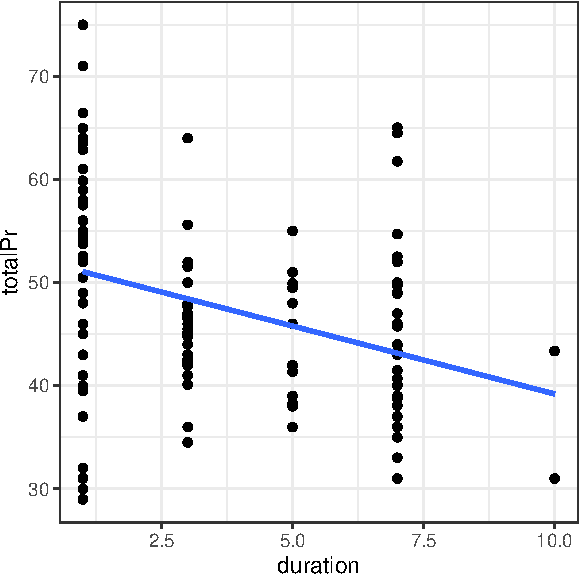
\includegraphics{MultLogSC_files/figure-latex/slrP1-1} 

}

\caption{`totalPr` versus `duration`}\label{fig:slrP1}
\end{figure}

\begin{itemize}
\tightlist
\item
  Fit a simple linear regression model for final auction price
  (\texttt{totalPr}) as a function of duration (\texttt{duration}).
\end{itemize}

\begin{Shaded}
\begin{Highlighting}[]
\CommentTok{# model with one slope}
\KeywordTok{lm}\NormalTok{(totalPr }\OperatorTok{~}\StringTok{ }\NormalTok{duration, }\DataTypeTok{data =}\NormalTok{ mario_kart)}
\end{Highlighting}
\end{Shaded}

\begin{verbatim}

Call:
lm(formula = totalPr ~ duration, data = mario_kart)

Coefficients:
(Intercept)     duration  
     52.374       -1.317  
\end{verbatim}

\begin{itemize}
\tightlist
\item
  Use \texttt{aes()} to add a color aesthetic that's mapped to the
  condition variable to the \texttt{slr} object, shown in Figure
  \ref{fig:slrP1}.
\end{itemize}

\begin{Shaded}
\begin{Highlighting}[]
\CommentTok{# plot with two slopes}
\NormalTok{slr }\OperatorTok{+}\StringTok{ }\KeywordTok{aes}\NormalTok{(}\DataTypeTok{color =}\NormalTok{ cond)}
\end{Highlighting}
\end{Shaded}

\begin{center}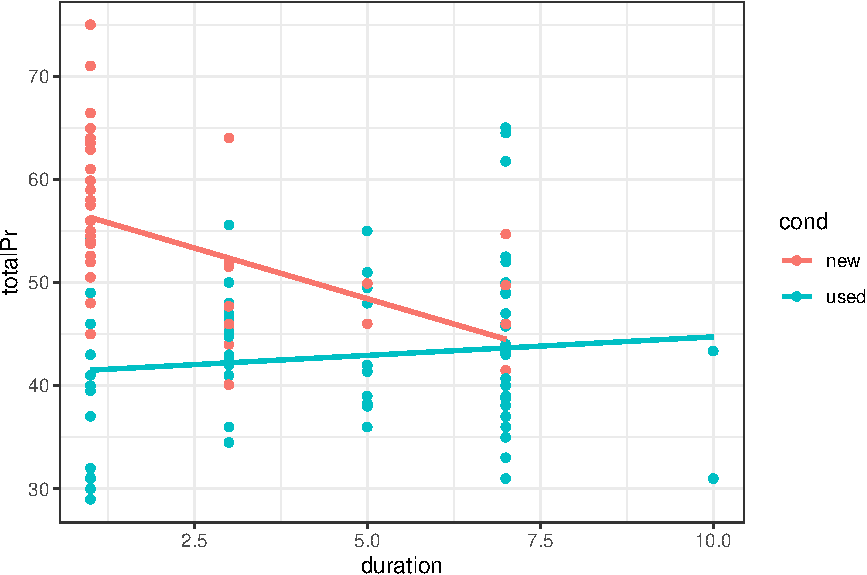
\includegraphics{MultLogSC_files/figure-latex/unnamed-chunk-24-1} \end{center}

\begin{itemize}
\tightlist
\item
  Which of the two groups is showing signs of Simpson's paradox?
  \textbf{Class discussion}
\end{itemize}

\begin{center}\rule{0.5\linewidth}{\linethickness}\end{center}

\chapter{Multiple Regression}\label{multiple-regression}

This chapter will show you how to add two, three, and even more numeric
explanatory variables to a linear model.

\section{Fitting a MLR model}\label{fitting-a-mlr-model}

In terms of the R code, fitting a multiple linear regression model is
easy: simply add variables to the model formula you specify in the
\texttt{lm()} command.

In a parallel slopes model, we had two explanatory variables: one was
numeric and one was categorical. Here, we will allow both explanatory
variables to be numeric.

\begin{center}\rule{0.5\linewidth}{\linethickness}\end{center}

\begin{Shaded}
\begin{Highlighting}[]
\KeywordTok{library}\NormalTok{(ggplot2)}
\KeywordTok{load}\NormalTok{(}\StringTok{"./Data/mario_kart.RData"}\NormalTok{)}
\KeywordTok{str}\NormalTok{(mario_kart)}
\end{Highlighting}
\end{Shaded}

\begin{verbatim}
'data.frame':   141 obs. of  12 variables:
 $ ID        : num  1.5e+11 2.6e+11 3.2e+11 2.8e+11 1.7e+11 ...
 $ duration  : int  3 7 3 3 1 3 1 1 3 7 ...
 $ nBids     : int  20 13 16 18 20 19 13 15 29 8 ...
 $ cond      : Factor w/ 2 levels "new","used": 1 2 1 1 1 1 2 1 2 2 ...
 $ startPr   : num  0.99 0.99 0.99 0.99 0.01 ...
 $ shipPr    : num  4 3.99 3.5 0 0 4 0 2.99 4 4 ...
 $ totalPr   : num  51.5 37 45.5 44 71 ...
 $ shipSp    : Factor w/ 8 levels "firstClass","media",..: 6 1 1 6 2 6 6 8 5 1 ...
 $ sellerRate: int  1580 365 998 7 820 270144 7284 4858 27 201 ...
 $ stockPhoto: Factor w/ 2 levels "no","yes": 2 2 1 2 2 2 2 2 2 1 ...
 $ wheels    : int  1 1 1 1 2 0 0 2 1 1 ...
 $ title     : Factor w/ 80 levels " Mario Kart Wii with Wii Wheel for Wii (New)",..: 80 60 22 7 4 19 34 5 79 70 ...
\end{verbatim}

The dataset \texttt{mario\_kart} is already loaded in your workspace.

\begin{itemize}
\tightlist
\item
  Fit a multiple linear regression model for total price as a function
  of the duration of the auction and the starting price.
\end{itemize}

\begin{Shaded}
\begin{Highlighting}[]
\CommentTok{# Fit the model using duration and startPr}
\NormalTok{mod <-}\StringTok{ }\KeywordTok{lm}\NormalTok{(totalPr }\OperatorTok{~}\StringTok{ }\NormalTok{duration }\OperatorTok{+}\StringTok{ }\NormalTok{startPr, }\DataTypeTok{data =}\NormalTok{ mario_kart)}
\NormalTok{mod}
\end{Highlighting}
\end{Shaded}

\begin{verbatim}

Call:
lm(formula = totalPr ~ duration + startPr, data = mario_kart)

Coefficients:
(Intercept)     duration      startPr  
     51.030       -1.508        0.233  
\end{verbatim}

\begin{center}\rule{0.5\linewidth}{\linethickness}\end{center}

\section{Tiling the plane}\label{tiling-the-plane}

One method for visualizing a multiple linear regression model is to
create a \href{https://en.wikipedia.org/wiki/Heat_map}{heatmap} of the
fitted values in the plane defined by the two explanatory variables.
This heatmap will illustrate how the model output changes over different
combinations of the explanatory variables.

This is a multistep process:

\begin{itemize}
\tightlist
\item
  First, create a grid of the possible pairs of values of the
  explanatory variables. The grid should be over the actual range of the
  data present in each variable. We've done this for you and stored the
  result as a data frame called \texttt{grid}.
\end{itemize}

\begin{Shaded}
\begin{Highlighting}[]
\NormalTok{grid <-}\StringTok{ }\KeywordTok{expand.grid}\NormalTok{(}\DataTypeTok{duration =} \KeywordTok{seq}\NormalTok{(}\DecValTok{1}\NormalTok{, }\DecValTok{10}\NormalTok{, }\DataTypeTok{by =} \DecValTok{1}\NormalTok{), }\DataTypeTok{startPr =} \KeywordTok{seq}\NormalTok{(}\FloatTok{0.01}\NormalTok{, }\FloatTok{69.95}\NormalTok{, }\DataTypeTok{by =} \FloatTok{0.01}\NormalTok{))}
\end{Highlighting}
\end{Shaded}

\begin{itemize}
\item
  Use \texttt{augment()} with the \texttt{newdata} argument to find the
  \(\hat{y}\)'s corresponding to the values in \texttt{grid}.
\item
  Add these to the \texttt{data\_space} plot by using the fill aesthetic
  and \texttt{geom\_tile()}.
\end{itemize}

\begin{Shaded}
\begin{Highlighting}[]
\NormalTok{data_space <-}\StringTok{ }\KeywordTok{ggplot}\NormalTok{(}\DataTypeTok{data =}\NormalTok{ mario_kart, }
                     \KeywordTok{aes}\NormalTok{(}\DataTypeTok{x =}\NormalTok{ duration, }\DataTypeTok{y =}\NormalTok{ startPr)) }\OperatorTok{+}\StringTok{ }
\StringTok{  }\KeywordTok{geom_point}\NormalTok{(}\KeywordTok{aes}\NormalTok{(}\DataTypeTok{color =}\NormalTok{ totalPr)) }\OperatorTok{+}\StringTok{ }
\StringTok{  }\KeywordTok{theme_bw}\NormalTok{()}
\NormalTok{data_space}
\end{Highlighting}
\end{Shaded}

\begin{center}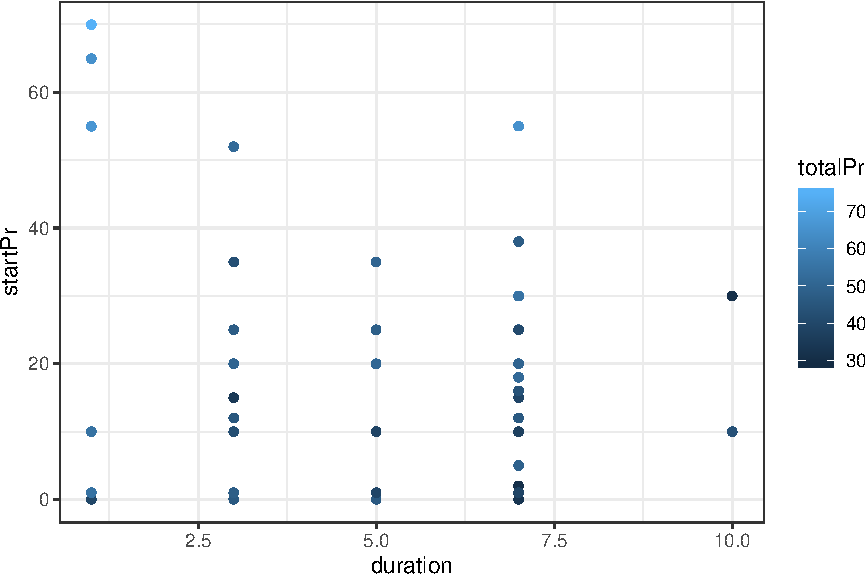
\includegraphics{MultLogSC_files/figure-latex/unnamed-chunk-28-1} \end{center}

\begin{center}\rule{0.5\linewidth}{\linethickness}\end{center}

\subsection*{Exercise}\label{exercise-9}
\addcontentsline{toc}{subsection}{Exercise}

The model object \texttt{mod} is already in your workspace.

\begin{itemize}
\tightlist
\item
  Use \texttt{augment()} to create a \texttt{data.frame} that contains
  the values the model outputs for each row of \texttt{grid}.
\end{itemize}

\begin{Shaded}
\begin{Highlighting}[]
\CommentTok{# add predictions to grid}
\NormalTok{price_hats <-}\StringTok{ }\NormalTok{broom}\OperatorTok{::}\KeywordTok{augment}\NormalTok{(mod, }\DataTypeTok{newdata =}\NormalTok{ grid)}
\end{Highlighting}
\end{Shaded}

\begin{itemize}
\tightlist
\item
  Use \texttt{geom\_tile} to illustrate these predicted values over the
  \texttt{data\_space} plot. Use the \texttt{fill} aesthetic and set
  \texttt{alpha\ =\ 0.5}.
\end{itemize}

\begin{Shaded}
\begin{Highlighting}[]
\CommentTok{# tile the plane}
\NormalTok{data_space }\OperatorTok{+}\StringTok{ }
\StringTok{   }\KeywordTok{geom_tile}\NormalTok{(}\DataTypeTok{data =}\NormalTok{ price_hats, }
             \KeywordTok{aes}\NormalTok{(}\DataTypeTok{fill =}\NormalTok{ .fitted), }\DataTypeTok{alpha =} \FloatTok{0.5}\NormalTok{)}
\end{Highlighting}
\end{Shaded}

\begin{center}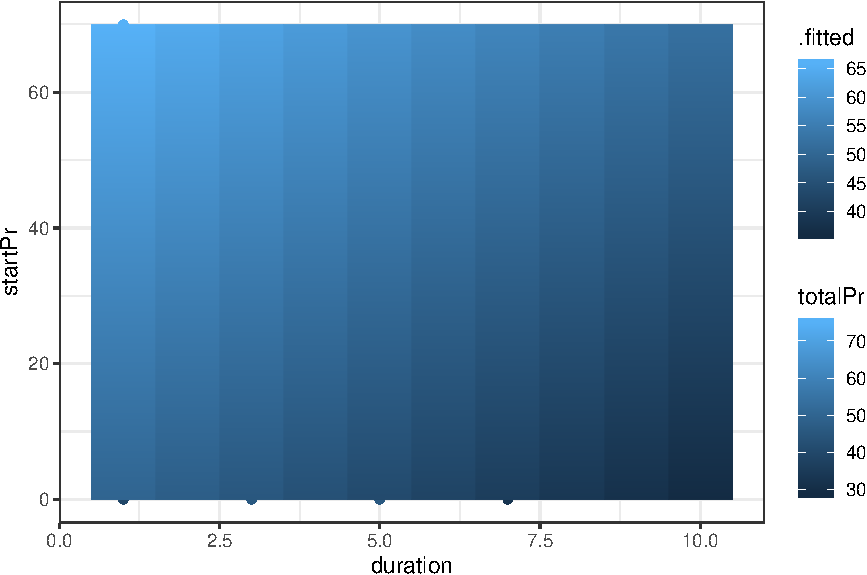
\includegraphics{MultLogSC_files/figure-latex/unnamed-chunk-30-1} \end{center}

\begin{center}\rule{0.5\linewidth}{\linethickness}\end{center}

\section{Models in 3D}\label{models-in-3d}

An alternative way to visualize a multiple regression model with two
numeric explanatory variables is as a plane in three dimensions. This is
possible in R using the \texttt{plotly} package.

We have created three objects that you will need:

\begin{itemize}
\tightlist
\item
  \texttt{x}: a vector of unique values of \texttt{duration}
\item
  \texttt{y}: a vector of unique values of \texttt{startPr}
\item
  \texttt{plane}: a matrix of the fitted values across all combinations
  of \texttt{x} and \texttt{y}
\end{itemize}

Much like \texttt{ggplot()}, the \texttt{plot\_ly()} function will allow
you to create a plot object with variables mapped to \texttt{x},
\texttt{y}, and \texttt{z} aesthetics. The \texttt{add\_markers()}
function is similar to \texttt{geom\_point()} in that it allows you to
add points to your 3D plot.

Note that \texttt{plot\_ly} uses the pipe (\texttt{\%\textgreater{}\%)}
operator to chain commands together.

\begin{center}\rule{0.5\linewidth}{\linethickness}\end{center}

\subsection*{Exercise}\label{exercise-10}
\addcontentsline{toc}{subsection}{Exercise}

\begin{itemize}
\tightlist
\item
  Run the \texttt{plot\_ly} command to draw 3D scatterplot for
  \texttt{totalPr} as a function of duration and \texttt{startPr} by
  mapping the \texttt{z} variable to the response and the \texttt{x} and
  \texttt{y} variables to the explanatory variables. Duration should be
  on the x-axis and starting price should be on the y-axis.
\end{itemize}

\begin{Shaded}
\begin{Highlighting}[]
\KeywordTok{library}\NormalTok{(plotly)}
\CommentTok{# draw the 3D scatterplot}
\NormalTok{p <-}\StringTok{ }\KeywordTok{plot_ly}\NormalTok{(}\DataTypeTok{data =}\NormalTok{ mario_kart, }\DataTypeTok{z =} \OperatorTok{~}\NormalTok{totalPr, }\DataTypeTok{x =} \OperatorTok{~}\NormalTok{duration, }\DataTypeTok{y =} \OperatorTok{~}\NormalTok{startPr, }\DataTypeTok{opacity =} \FloatTok{0.6}\NormalTok{) }\OperatorTok
\StringTok{  }\KeywordTok{add_markers}\NormalTok{() }
\NormalTok{p}
\end{Highlighting}
\end{Shaded}

\hypertarget{htmlwidget-b1a075f5538d7f834f47}{}

\begin{itemize}
\tightlist
\item
  Use \texttt{add\_surface()} to draw a plane through the cloud of
  points by setting \texttt{z\ =\ \textasciitilde{}plane}. See
  \href{https://en.wikipedia.org/wiki/Outer_product}{wikipedia} for the
  definition of an outer product. In what follows, we will use the R
  function \texttt{outer()} to compute the values of \texttt{plane}.
\end{itemize}

\[\bf{u \otimes v} = \bf{uv^T}\]

\begin{Shaded}
\begin{Highlighting}[]
\KeywordTok{summary}\NormalTok{(mod)}\OperatorTok{$}\NormalTok{coef}
\end{Highlighting}
\end{Shaded}

\begin{verbatim}
              Estimate Std. Error   t value     Pr(>|t|)
(Intercept) 51.0295070 1.17913685 43.277001 3.665684e-82
duration    -1.5081260 0.25551997 -5.902184 2.644972e-08
startPr      0.2329542 0.04363644  5.338525 3.755647e-07
\end{verbatim}

\begin{Shaded}
\begin{Highlighting}[]
\NormalTok{x <-}\StringTok{ }\KeywordTok{seq}\NormalTok{(}\DecValTok{1}\NormalTok{, }\DecValTok{10}\NormalTok{, }\DataTypeTok{length =} \DecValTok{70}\NormalTok{)}
\NormalTok{y <-}\StringTok{ }\KeywordTok{seq}\NormalTok{(}\FloatTok{0.010}\NormalTok{, }\FloatTok{59.950}\NormalTok{, }\DataTypeTok{length =} \DecValTok{70}\NormalTok{)}
\NormalTok{plane <-}\StringTok{ }\KeywordTok{outer}\NormalTok{(x, y, }\ControlFlowTok{function}\NormalTok{(a, b)\{}\KeywordTok{summary}\NormalTok{(mod)}\OperatorTok{$}\NormalTok{coef[}\DecValTok{1}\NormalTok{,}\DecValTok{1}\NormalTok{] }\OperatorTok{+}\StringTok{ }
\StringTok{    }\KeywordTok{summary}\NormalTok{(mod)}\OperatorTok{$}\NormalTok{coef[}\DecValTok{2}\NormalTok{,}\DecValTok{1}\NormalTok{]}\OperatorTok{*}\NormalTok{a }\OperatorTok{+}\StringTok{ }\KeywordTok{summary}\NormalTok{(mod)}\OperatorTok{$}\NormalTok{coef[}\DecValTok{3}\NormalTok{,}\DecValTok{1}\NormalTok{]}\OperatorTok{*}\NormalTok{b\})}
\CommentTok{# draw the plane}
\NormalTok{p }\OperatorTok
\StringTok{  }\KeywordTok{add_surface}\NormalTok{(}\DataTypeTok{x =} \OperatorTok{~}\NormalTok{x, }\DataTypeTok{y =} \OperatorTok{~}\NormalTok{y, }\DataTypeTok{z =} \OperatorTok{~}\NormalTok{plane, }\DataTypeTok{showscale =} \OtherTok{FALSE}\NormalTok{)}
\end{Highlighting}
\end{Shaded}

\hypertarget{htmlwidget-7a63ded58c7f2591b816}{}

\begin{center}\rule{0.5\linewidth}{\linethickness}\end{center}

\subsection*{Coefficient magnitude}\label{coefficient-magnitude}
\addcontentsline{toc}{subsection}{Coefficient magnitude}

The coefficients from our model for the total auction price of
MarioKarts as a function of auction duration and starting price are
shown below.

\begin{Shaded}
\begin{Highlighting}[]
\NormalTok{mod}
\end{Highlighting}
\end{Shaded}

\begin{verbatim}

Call:
lm(formula = totalPr ~ duration + startPr, data = mario_kart)

Coefficients:
(Intercept)     duration      startPr  
     51.030       -1.508        0.233  
\end{verbatim}

A colleague claims that these results imply that the duration of the
auction is a more important determinant of final price than starting
price, because the coefficient is larger. This interpretation is false
because:

\begin{center}\rule{0.5\linewidth}{\linethickness}\end{center}

\begin{itemize}
\item
  The coefficient on duration is negative.
\item
  Smaller coefficients are more important.
\item
  \textbf{The coefficients have different units (dollars per day and
  dollars per dollar, respectively) and so they are not directly
  comparable.}
\item
  The intercept coefficient is much bigger, so it is the most important
  one.
\end{itemize}

\begin{center}\rule{0.5\linewidth}{\linethickness}\end{center}

\subsection*{Practicing interpretation}\label{practicing-interpretation}
\addcontentsline{toc}{subsection}{Practicing interpretation}

Fit a multiple regression model for the total auction price of an item
in the \texttt{mario\_kart} data set as a function of the starting price
and the duration of the auction. Compute the coefficients and choose the
correct interpretation of the duration variable.

\begin{center}\rule{0.5\linewidth}{\linethickness}\end{center}

\begin{itemize}
\item
  \textbf{For each additional day the auction lasts, the expected final
  price declines by \$1.51, after controlling for starting price.}
\item
  For each additional dollar of starting price, the expected final price
  increases by \$0.23, after controlling for the duration of the
  auction.
\item
  The duration of the auction is a more important determinant of final
  price than starting price, because the coefficient is larger.
\item
  The average auction lasts 51 days.
\end{itemize}

\begin{center}\rule{0.5\linewidth}{\linethickness}\end{center}

\section{Visualizing parallel planes}\label{visualizing-parallel-planes}

By including the duration, starting price, and condition variables in
our model, we now have two explanatory variables and one categorical
variable. Our model now takes the geometric form of two parallel planes!

The first plane corresponds to the model output when the condition of
the item is \texttt{new}, while the second plane corresponds to the
model output when the condition of the item is \texttt{used}. The planes
have the same slopes along both the duration and starting price
axes---it is the z-intercept that is different.

Once again we have stored the \texttt{x} and \texttt{y} vectors for you.
Since we now have two planes, there are matrix objects \texttt{plane0}
and \texttt{plane1} stored for you as well.

\begin{Shaded}
\begin{Highlighting}[]
\NormalTok{modI <-}\StringTok{ }\KeywordTok{lm}\NormalTok{(totalPr }\OperatorTok{~}\StringTok{ }\NormalTok{duration }\OperatorTok{+}\StringTok{ }\NormalTok{startPr }\OperatorTok{+}\StringTok{ }\NormalTok{cond, }\DataTypeTok{data =}\NormalTok{ mario_kart)}
\KeywordTok{summary}\NormalTok{(modI)}\OperatorTok{$}\NormalTok{coef}
\end{Highlighting}
\end{Shaded}

\begin{verbatim}
              Estimate Std. Error   t value     Pr(>|t|)
(Intercept) 53.3447530  1.0804915 49.370822 3.781243e-89
duration    -0.6559841  0.2553503 -2.568957 1.127073e-02
startPr      0.1981653  0.0382717  5.177855 7.835882e-07
condused    -8.9493214  1.3237851 -6.760403 3.635333e-10
\end{verbatim}

\begin{Shaded}
\begin{Highlighting}[]
\NormalTok{plane0 <-}\StringTok{ }\KeywordTok{outer}\NormalTok{(x, y, }\ControlFlowTok{function}\NormalTok{(a, b)\{}\FloatTok{53.3447530} \OperatorTok{-}\FloatTok{0.6559841}\OperatorTok{*}\NormalTok{a }\OperatorTok{+}\StringTok{ }
\StringTok{                                      }\FloatTok{0.1981653}\OperatorTok{*}\NormalTok{b\})}
\NormalTok{plane1 <-}\StringTok{ }\KeywordTok{outer}\NormalTok{(x, y, }\ControlFlowTok{function}\NormalTok{(a, b)\{}\FloatTok{53.3447530} \OperatorTok{-}\FloatTok{0.6559841}\OperatorTok{*}\NormalTok{a }\OperatorTok{+}
\StringTok{                                      }\FloatTok{0.1981653}\OperatorTok{*}\NormalTok{b }\OperatorTok{-}\StringTok{ }\FloatTok{8.9493214}\NormalTok{\})}
\end{Highlighting}
\end{Shaded}

\begin{center}\rule{0.5\linewidth}{\linethickness}\end{center}

\subsection*{Exercise}\label{exercise-11}
\addcontentsline{toc}{subsection}{Exercise}

\begin{itemize}
\tightlist
\item
  Use \texttt{plot\_ly} to draw 3D scatterplot for \texttt{totalPr} as a
  function of \texttt{duration}, \texttt{startPr}, and \texttt{cond} by
  mapping the \texttt{z} variable to the response and the \texttt{x} and
  \texttt{y} variables to the explanatory variables. Duration should be
  on the x-axis and starting price should be on the y-axis. Use color to
  represent \texttt{cond}.
\end{itemize}

\begin{Shaded}
\begin{Highlighting}[]
\CommentTok{# draw the 3D scatterplot}
\NormalTok{p <-}\StringTok{ }\KeywordTok{plot_ly}\NormalTok{(}\DataTypeTok{data =}\NormalTok{ mario_kart, }\DataTypeTok{z =} \OperatorTok{~}\NormalTok{totalPr, }\DataTypeTok{x =} \OperatorTok{~}\NormalTok{duration, }\DataTypeTok{y =} \OperatorTok{~}\NormalTok{startPr, }\DataTypeTok{opacity =} \FloatTok{0.6}\NormalTok{) }\OperatorTok
\StringTok{  }\KeywordTok{add_markers}\NormalTok{(}\DataTypeTok{color =} \OperatorTok{~}\NormalTok{cond) }
\NormalTok{p}
\end{Highlighting}
\end{Shaded}

\hypertarget{htmlwidget-358eeb0b2e917045f18e}{}

\begin{itemize}
\tightlist
\item
  Use \texttt{add\_surface()} (twice) to draw two planes through the
  cloud of points, one for new MarioKarts and another for used ones. Use
  the objects \texttt{plane0} and \texttt{plane1}.
\end{itemize}

\begin{Shaded}
\begin{Highlighting}[]
\CommentTok{# draw two planes}
\NormalTok{p }\OperatorTok
\StringTok{  }\KeywordTok{add_surface}\NormalTok{(}\DataTypeTok{x =} \OperatorTok{~}\NormalTok{x, }\DataTypeTok{y =} \OperatorTok{~}\NormalTok{y, }\DataTypeTok{z =} \OperatorTok{~}\NormalTok{plane0, }\DataTypeTok{showscale =} \OtherTok{FALSE}\NormalTok{) }\OperatorTok
\StringTok{  }\KeywordTok{add_surface}\NormalTok{(}\DataTypeTok{x =} \OperatorTok{~}\NormalTok{x, }\DataTypeTok{y =} \OperatorTok{~}\NormalTok{y, }\DataTypeTok{z =} \OperatorTok{~}\NormalTok{plane1, }\DataTypeTok{showscale =} \OtherTok{FALSE}\NormalTok{)}
\end{Highlighting}
\end{Shaded}

\hypertarget{htmlwidget-8a6c2d5675e6f40c5e57}{}

\begin{center}\rule{0.5\linewidth}{\linethickness}\end{center}

\subsection*{Parallel plane
interpretation}\label{parallel-plane-interpretation}
\addcontentsline{toc}{subsection}{Parallel plane interpretation}

The coefficients from our parallel planes model is shown below.

\begin{Shaded}
\begin{Highlighting}[]
\NormalTok{modI}
\end{Highlighting}
\end{Shaded}

\begin{verbatim}

Call:
lm(formula = totalPr ~ duration + startPr + cond, data = mario_kart)

Coefficients:
(Intercept)     duration      startPr     condused  
    53.3448      -0.6560       0.1982      -8.9493  
\end{verbatim}

Choose the right interpretation of \(\beta_3\) (the coefficient on
\texttt{condUsed}):

\begin{center}\rule{0.5\linewidth}{\linethickness}\end{center}

\begin{itemize}
\item
  \textbf{The expected premium for new (relative to used) MarioKarts is
  \$8.95, after controlling for the duration and starting price of the
  auction.}
\item
  The expected premium for used (relative to new) MarioKarts is \$8.95,
  after controlling for the duration and starting price of the auction.
\item
  For each additional day the auction lasts, the expected final price
  declines by \$8.95, after controlling for starting price and
  condition.
\end{itemize}

\begin{center}\rule{0.5\linewidth}{\linethickness}\end{center}

\subsection*{Interpretation of coefficient in a big
model}\label{interpretation-of-coefficient-in-a-big-model}
\addcontentsline{toc}{subsection}{Interpretation of coefficient in a big
model}

This time we have thrown even more variables into our model, including
the number of bids in each auction (\texttt{nBids}) and the number of
wheels. Unfortunately this makes a full visualization of our model
impossible, but we can still interpret the coefficients.

\begin{Shaded}
\begin{Highlighting}[]
\NormalTok{modJ <-}\StringTok{ }\KeywordTok{lm}\NormalTok{(totalPr }\OperatorTok{~}\StringTok{ }\NormalTok{duration }\OperatorTok{+}\StringTok{ }\NormalTok{startPr }\OperatorTok{+}\StringTok{ }\NormalTok{cond }\OperatorTok{+}\StringTok{ }\NormalTok{wheels }\OperatorTok{+}\StringTok{ }\NormalTok{nBids, }
    \DataTypeTok{data =}\NormalTok{ mario_kart)}
\NormalTok{modJ}
\end{Highlighting}
\end{Shaded}

\begin{verbatim}

Call:
lm(formula = totalPr ~ duration + startPr + cond + wheels + nBids, 
    data = mario_kart)

Coefficients:
(Intercept)     duration      startPr     condused       wheels  
    39.3741      -0.2752       0.1796      -4.7720       6.7216  
      nBids  
     0.1909  
\end{verbatim}

Choose the correct interpretation of the coefficient on the number of
wheels:

\begin{center}\rule{0.5\linewidth}{\linethickness}\end{center}

\begin{itemize}
\item
  The average number of wheels is 6.72.
\item
  Each additional wheel costs exactly \$6.72.
\item
  Each additional wheel is associated with an increase in the expected
  auction price of \$6.72.
\item
  \textbf{Each additional wheel is associated with an increase in the
  expected auction price of \$6.72, after controlling for auction
  duration, starting price, number of bids, and the condition of the
  item.}
\end{itemize}

\begin{center}\rule{0.5\linewidth}{\linethickness}\end{center}

\chapter{Logistic Regression}\label{logistic-regression}

n this chapter you'll learn about using logistic regression, a
generalized linear model (GLM), to predict a binary outcome and classify
observations.

\begin{center}\rule{0.5\linewidth}{\linethickness}\end{center}

\section{Fitting a line to a binary
response}\label{fitting-a-line-to-a-binary-response}

When our response variable is binary, a regression model has several
limitations. Among the more obvious---and logically incongruous---is
that the regression line extends infinitely in either direction. This
means that even though our response variable \(y\) only takes on the
values 0 and 1, our fitted values \(\hat{y}\) can range anywhere from
\(-\infty\) to \(\infty\). This doesn't make sense.

To see this in action, we'll fit a linear regression model to data about
55 students who applied to medical school. We want to understand how
their undergraduate GPA relates to the probability they will be accepted
by a particular school (\texttt{Acceptance}).

\begin{center}\rule{0.5\linewidth}{\linethickness}\end{center}

\subsection*{Exercise}\label{exercise-12}
\addcontentsline{toc}{subsection}{Exercise}

\begin{Shaded}
\begin{Highlighting}[]
\KeywordTok{library}\NormalTok{(Stat2Data)}
\KeywordTok{data}\NormalTok{(MedGPA)}
\end{Highlighting}
\end{Shaded}

The medical school acceptance data is loaded in your workspace as
\texttt{MedGPA}.

\begin{itemize}
\tightlist
\item
  Create a scatterplot called \texttt{data\_space} for
  \texttt{Acceptance} as a function of \texttt{GPA}. Use
  \texttt{geom\_jitter()} to apply a small amount of jitter to the
  points in the y-direction by setting \texttt{width\ =\ 0} and
  \texttt{height\ =\ 0.05}.
\end{itemize}

\begin{Shaded}
\begin{Highlighting}[]
\CommentTok{# scatterplot with jitter}
\NormalTok{data_space <-}\StringTok{ }\KeywordTok{ggplot}\NormalTok{(}\DataTypeTok{data =}\NormalTok{ MedGPA, }\KeywordTok{aes}\NormalTok{(}\DataTypeTok{x =}\NormalTok{ GPA, }\DataTypeTok{y =}\NormalTok{ Acceptance)) }\OperatorTok{+}
\StringTok{  }\KeywordTok{geom_jitter}\NormalTok{(}\DataTypeTok{width =} \DecValTok{0}\NormalTok{, }\DataTypeTok{height =} \FloatTok{0.05}\NormalTok{, }\DataTypeTok{alpha =} \FloatTok{0.5}\NormalTok{) }\OperatorTok{+}\StringTok{ }
\StringTok{  }\KeywordTok{theme_bw}\NormalTok{()}
\NormalTok{data_space}
\end{Highlighting}
\end{Shaded}

\begin{center}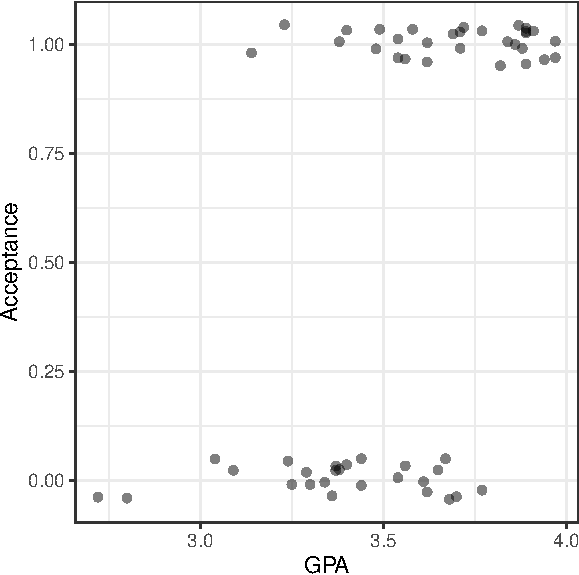
\includegraphics{MultLogSC_files/figure-latex/unnamed-chunk-41-1} \end{center}

\begin{itemize}
\tightlist
\item
  Use \texttt{geom\_smooth()} to add the simple linear regression line
  to \texttt{data\_space}.
\end{itemize}

\begin{Shaded}
\begin{Highlighting}[]
\CommentTok{# linear regression line}
\NormalTok{data_space }\OperatorTok{+}\StringTok{ }
\StringTok{  }\KeywordTok{geom_smooth}\NormalTok{(}\DataTypeTok{method =} \StringTok{"lm"}\NormalTok{, }\DataTypeTok{se =} \OtherTok{FALSE}\NormalTok{)}
\end{Highlighting}
\end{Shaded}

\begin{center}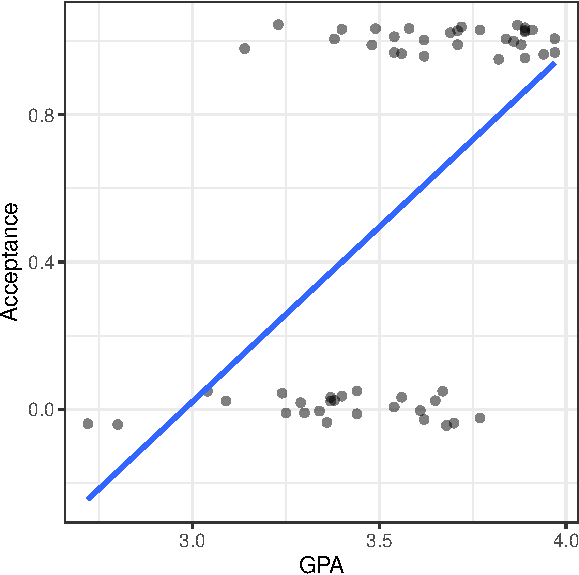
\includegraphics{MultLogSC_files/figure-latex/unnamed-chunk-42-1} \end{center}

\begin{center}\rule{0.5\linewidth}{\linethickness}\end{center}

\section{Fitting a line to a binary response
(2)}\label{fitting-a-line-to-a-binary-response-2}

In the previous exercise, we identified a major limitation to fitting a
linear regression model when we have a binary response variable.
However, it is not always inappropriate to do so. Note that our
regression line only makes illogical predictions (i.e. \(\hat{y} < 0\)
or \(\hat{y} > 1\)) for students with very high or very low GPAs. For
GPAs closer to average, the predictions seem fine.

Moreover, the alternative logistic regression model---which we will fit
next---is very similar to the linear regression model for observations
near the average of the explanatory variable. It just so happens that
the logistic curve is very straight near its middle. Thus, in these
cases a linear regression model may still be acceptable, even for a
binary response.

\begin{center}\rule{0.5\linewidth}{\linethickness}\end{center}

\subsection*{Exercise}\label{exercise-13}
\addcontentsline{toc}{subsection}{Exercise}

\begin{itemize}
\tightlist
\item
  Use \texttt{filter()} to find the subset of the observations whose
  GPAs are between 3.375 and 3.77, inclusive.
\end{itemize}

\begin{Shaded}
\begin{Highlighting}[]
\CommentTok{# filter}
\NormalTok{MedGPA_middle <-}\StringTok{ }\KeywordTok{filter}\NormalTok{(MedGPA, GPA }\OperatorTok{>=}\StringTok{ }\FloatTok{3.375}\NormalTok{, GPA }\OperatorTok{<=}\StringTok{ }\FloatTok{3.77}\NormalTok{)}
\KeywordTok{head}\NormalTok{(MedGPA_middle)}
\end{Highlighting}
\end{Shaded}

\begin{verbatim}
  Accept Acceptance Sex BCPM  GPA VR PS WS BS MCAT Apps
1      D          0   F 3.59 3.62 11  9  9  9   38    5
2      A          1   F 3.74 3.69 12 11  7 10   40    5
3      A          1   F 3.53 3.38  9 11  4 11   35   11
4      A          1   M 3.59 3.72 10  9  7 10   36    5
5      A          1   F 3.74 3.71  8 10  6 11   35    5
6      A          1   F 3.35 3.49 11  8  4  8   31    9
\end{verbatim}

\begin{itemize}
\tightlist
\item
  Create a scatterplot called data\_space for Acceptance as a function
  of GPA for only those observations. Use geom\_jitter() to apply 0.05
  jitter to the points in the \(y\)-direction and no jitter to the
  \(x\)-direction.
\end{itemize}

\begin{Shaded}
\begin{Highlighting}[]
\CommentTok{# scatterplot with jitter}
\NormalTok{data_space <-}\StringTok{ }\KeywordTok{ggplot}\NormalTok{(MedGPA_middle, }\KeywordTok{aes}\NormalTok{(}\DataTypeTok{x =}\NormalTok{ GPA, }\DataTypeTok{y =}\NormalTok{ Acceptance)) }\OperatorTok{+}\StringTok{ }
\StringTok{  }\KeywordTok{geom_jitter}\NormalTok{(}\DataTypeTok{width =} \DecValTok{0}\NormalTok{, }\DataTypeTok{height =} \FloatTok{0.05}\NormalTok{, }\DataTypeTok{alpha =} \FloatTok{0.5}\NormalTok{) }\OperatorTok{+}\StringTok{ }
\StringTok{  }\KeywordTok{theme_bw}\NormalTok{()}
\NormalTok{data_space}
\end{Highlighting}
\end{Shaded}

\begin{center}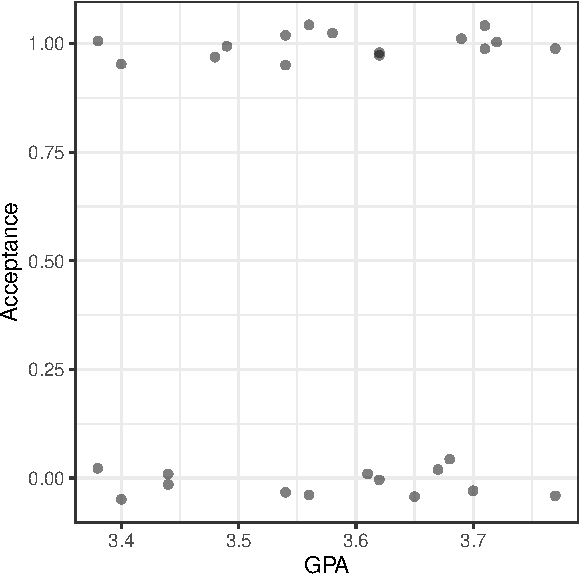
\includegraphics{MultLogSC_files/figure-latex/unnamed-chunk-44-1} \end{center}

\begin{itemize}
\tightlist
\item
  Use geom\_smooth() to add only the simple linear regression line to
  data\_space.
\end{itemize}

\begin{Shaded}
\begin{Highlighting}[]
\CommentTok{# linear regression line}
\NormalTok{data_space }\OperatorTok{+}\StringTok{ }
\StringTok{  }\KeywordTok{geom_smooth}\NormalTok{(}\DataTypeTok{method =} \StringTok{"lm"}\NormalTok{, }\DataTypeTok{se =} \OtherTok{FALSE}\NormalTok{)}
\end{Highlighting}
\end{Shaded}

\begin{center}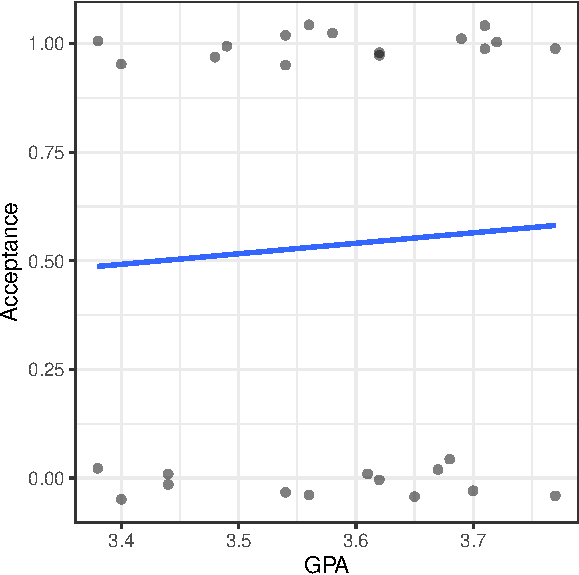
\includegraphics{MultLogSC_files/figure-latex/unnamed-chunk-45-1} \end{center}

\begin{center}\rule{0.5\linewidth}{\linethickness}\end{center}

\section{Fitting a model}\label{fitting-a-model}

Logistic regression is a special case of a broader class of
\href{https://en.wikipedia.org/wiki/Generalized_linear_model}{generalized
linear models}, often known as GLMs. Specifying a logistic regression
model is very similar to specify a regression model, with two important
differences:

\begin{itemize}
\item
  We use the \texttt{glm()} function instead of \texttt{lm()}
\item
  We specify the \texttt{family} argument and set it to
  \texttt{binomial}. This tells the GLM function that we want to fit a
  logistic regression model to our binary response.
  \href{https://en.wikipedia.org/wiki/Binomial_distribution}{The
  terminology stems from the assumption that our binary response follows
  a \{binomial distribution.}
\end{itemize}

We still use the formula and data arguments with \texttt{glm()}.

Note that the mathematical model is now:

\begin{equation}
\log\left(\frac{y}{1-y}\right) = \beta_0 + \beta_1 \cdot x + \varepsilon,
\end{equation}

where \(\varepsilon\) is the error term.

\begin{center}\rule{0.5\linewidth}{\linethickness}\end{center}

\subsection*{Exercise}\label{exercise-14}
\addcontentsline{toc}{subsection}{Exercise}

\begin{itemize}
\tightlist
\item
  Use \texttt{glm()} to fit a logistic regression model for
  \texttt{Acceptance} as a function of \texttt{GPA}.
\end{itemize}

\begin{Shaded}
\begin{Highlighting}[]
\CommentTok{# fit model}
\NormalTok{mod <-}\StringTok{ }\KeywordTok{glm}\NormalTok{(Acceptance }\OperatorTok{~}\StringTok{ }\NormalTok{GPA, }\DataTypeTok{data =}\NormalTok{ MedGPA, }\DataTypeTok{family =}\NormalTok{ binomial)}
\NormalTok{mod}
\end{Highlighting}
\end{Shaded}

\begin{verbatim}

Call:  glm(formula = Acceptance ~ GPA, family = binomial, data = MedGPA)

Coefficients:
(Intercept)          GPA  
    -19.207        5.454  

Degrees of Freedom: 54 Total (i.e. Null);  53 Residual
Null Deviance:      75.79 
Residual Deviance: 56.84    AIC: 60.84
\end{verbatim}

\begin{center}\rule{0.5\linewidth}{\linethickness}\end{center}

\section{Using geom\_smooth()}\label{using-geom_smooth}

Our logistic regression model can be visualized in the data space by
overlaying the appropriate logistic curve. We can use the
\texttt{geom\_smooth()} function to do this. Recall that
\texttt{geom\_smooth()} takes a method argument that allows you to
specify what type of smoother you want to see. In our case, we need to
specify that we want to use the \texttt{glm()} function to do the
smoothing.

However we also need to tell the \texttt{glm()} function which member of
the GLM family we want to use. To do this, we will pass the
\texttt{family} argument to \texttt{glm()} as a list using the
\texttt{method.args} argument to \texttt{geom\_smooth()}. This mechanism
is common in R, and allows one function to pass a list of arguments to
another function.

\begin{center}\rule{0.5\linewidth}{\linethickness}\end{center}

\subsection*{Exercise}\label{exercise-15}
\addcontentsline{toc}{subsection}{Exercise}

\begin{itemize}
\tightlist
\item
  Create a scatterplot called \texttt{data\_space} for
  \texttt{Acceptance} as a function of \texttt{GPA}. Use
  \texttt{geom\_jitter()} to apply a small amount of jitter to the
  points in the \(y\)-direction. Set \texttt{width\ =\ 0} and
  \texttt{height\ =\ 0.05} in \texttt{geom\_jitter()}.
\end{itemize}

\begin{Shaded}
\begin{Highlighting}[]
\CommentTok{# scatterplot with jitter}
\NormalTok{data_space <-}\StringTok{ }\KeywordTok{ggplot}\NormalTok{(}\DataTypeTok{data =}\NormalTok{ MedGPA, }\KeywordTok{aes}\NormalTok{(}\DataTypeTok{y =}\NormalTok{ Acceptance, }\DataTypeTok{x =}\NormalTok{ GPA)) }\OperatorTok{+}\StringTok{ }
\StringTok{  }\KeywordTok{geom_jitter}\NormalTok{(}\DataTypeTok{width =} \DecValTok{0}\NormalTok{, }\DataTypeTok{height =} \FloatTok{0.05}\NormalTok{, }\DataTypeTok{alpha =} \FloatTok{0.5}\NormalTok{) }\OperatorTok{+}\StringTok{ }
\StringTok{  }\KeywordTok{theme_bw}\NormalTok{()}
\end{Highlighting}
\end{Shaded}

\begin{itemize}
\tightlist
\item
  Use \texttt{geom\_smooth()} to add the logistic regression line to
  \texttt{data\_space} by specifying the \texttt{method} and
  \texttt{method.args} arguments to fit a logistic \texttt{glm}.
\end{itemize}

\begin{Shaded}
\begin{Highlighting}[]
\CommentTok{# add logistic curve}
\NormalTok{data_space }\OperatorTok{+}
\StringTok{  }\KeywordTok{geom_smooth}\NormalTok{(}\DataTypeTok{method =} \StringTok{"glm"}\NormalTok{, }\DataTypeTok{se =} \OtherTok{FALSE}\NormalTok{, }\DataTypeTok{method.args =} \KeywordTok{list}\NormalTok{(}\DataTypeTok{family =} \StringTok{"binomial"}\NormalTok{))}
\end{Highlighting}
\end{Shaded}

\begin{center}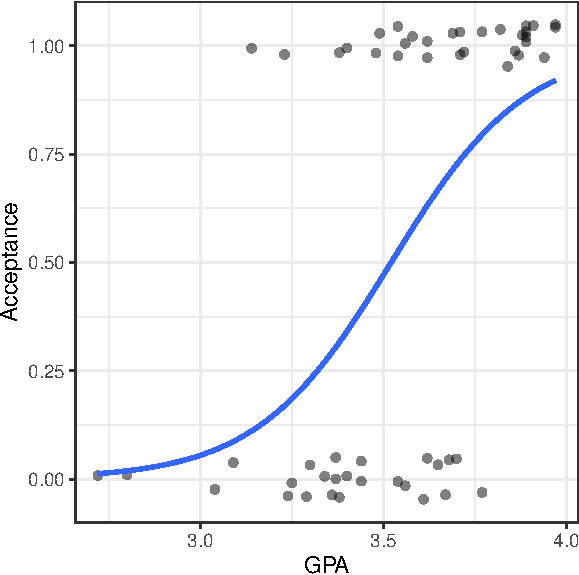
\includegraphics{MultLogSC_files/figure-latex/unnamed-chunk-48-1} \end{center}

\begin{center}\rule{0.5\linewidth}{\linethickness}\end{center}

\section{Using bins}\label{using-bins}

One of the difficulties in working with a binary response variable is
understanding how it ``changes.'' The response itself (\(y\)) is either
0 or 1, while the fitted values (\(\hat{y}\))---which are interpreted as
probabilities---are between 0 and 1. But if every medical school
applicant is either admitted or not, what does it mean to talk about the
probability of being accepted?

What we'd like is a larger sample of students, so that for each GPA
value (e.g.~3.54) we had many observations (say \(n\)), and we could
then take the average of those \(n\) observations to arrive at the
estimated probability of acceptance. Unfortunately, since the
explanatory variable is continuous, this is hopeless---it would take an
infinite amount of data to make these estimates robust.

Instead, what we can do is put the observations into bins based on their
GPA value. Within each bin, we can compute the proportion of accepted
students, and we can visualize our model as a smooth logistic curve
through those binned values.

We have created a \texttt{data.frame} called \texttt{MedGPA\_binned}
that aggregates the original data into separate bins for each
\textbf{1/6} of GPA. It also contains the fitted values from the
logistic regression model.

\begin{Shaded}
\begin{Highlighting}[]
\NormalTok{gpa_bins <-}\StringTok{ }\KeywordTok{quantile}\NormalTok{(MedGPA}\OperatorTok{$}\NormalTok{GPA, }\DataTypeTok{probs =} \KeywordTok{seq}\NormalTok{(}\DecValTok{0}\NormalTok{, }\DecValTok{1}\NormalTok{, }\DecValTok{1}\OperatorTok{/}\DecValTok{6}\NormalTok{))}
\NormalTok{gpa_bins}
\end{Highlighting}
\end{Shaded}

\begin{verbatim}
       0% 16.66667% 33.33333%       50% 66.66667% 83.33333%      100% 
     2.72      3.30      3.44      3.58      3.70      3.87      3.97 
\end{verbatim}

\begin{Shaded}
\begin{Highlighting}[]
\NormalTok{MedGPA}\OperatorTok{$}\NormalTok{bins <-}\StringTok{ }\KeywordTok{cut}\NormalTok{(MedGPA}\OperatorTok{$}\NormalTok{GPA, }\DataTypeTok{breaks =}\NormalTok{ gpa_bins, }\DataTypeTok{include.lowest =} \OtherTok{TRUE}\NormalTok{)}
\KeywordTok{head}\NormalTok{(MedGPA)}
\end{Highlighting}
\end{Shaded}

\begin{verbatim}
  Accept Acceptance Sex BCPM  GPA VR PS WS BS MCAT Apps       bins
1      D          0   F 3.59 3.62 11  9  9  9   38    5 (3.58,3.7]
2      A          1   M 3.75 3.84 12 13  8 12   45    3 (3.7,3.87]
3      A          1   F 3.24 3.23  9 10  5  9   33   19 [2.72,3.3]
4      A          1   F 3.74 3.69 12 11  7 10   40    5 (3.58,3.7]
5      A          1   F 3.53 3.38  9 11  4 11   35   11 (3.3,3.44]
6      A          1   M 3.59 3.72 10  9  7 10   36    5 (3.7,3.87]
\end{verbatim}

\begin{Shaded}
\begin{Highlighting}[]
\NormalTok{MedGPA_binned <-}\StringTok{ }\NormalTok{MedGPA }\OperatorTok\StringTok{ }
\StringTok{  }\KeywordTok{group_by}\NormalTok{(bins) }\OperatorTok\StringTok{ }
\StringTok{  }\KeywordTok{summarize}\NormalTok{(}\DataTypeTok{mean_GPA =} \KeywordTok{mean}\NormalTok{(GPA), }\DataTypeTok{acceptance_rate =} \KeywordTok{mean}\NormalTok{(Acceptance))}
\NormalTok{MedGPA_binned}
\end{Highlighting}
\end{Shaded}

\begin{verbatim}
# A tibble: 6 x 3
  bins        mean_GPA acceptance_rate
  <fct>          <dbl>           <dbl>
1 [2.72,3.3]      3.11           0.2  
2 (3.3,3.44]      3.39           0.2  
3 (3.44,3.58]     3.54           0.75 
4 (3.58,3.7]      3.65           0.333
5 (3.7,3.87]      3.79           0.889
6 (3.87,3.97]     3.91           1    
\end{verbatim}

Here we are plotting \(y\) as a function of \(x\), where that function
is

\begin{equation}
\hat{p}(X) = \widehat{\text{Pr}}(Y=1|X) = \frac{\exp(\hat{\beta}_0 + \hat{\beta}_1 x)}{1 + \exp(\hat{\beta}_0 + \hat{\beta}_1 x)}
\end{equation}

Note that the left hand side is the expected probability \(y\) of being
accepted to medical school.

\begin{center}\rule{0.5\linewidth}{\linethickness}\end{center}

\subsection*{Exercise}\label{exercise-16}
\addcontentsline{toc}{subsection}{Exercise}

\begin{itemize}
\tightlist
\item
  Create a scatterplot called \texttt{data\_space} for
  \texttt{acceptance\_rate} as a function of \texttt{mean\_GPA} using
  the binned data in \texttt{MedGPA\_binned}. Use \texttt{geom\_line()}
  to connect the points.
\end{itemize}

\begin{Shaded}
\begin{Highlighting}[]
\CommentTok{# binned points and line}
\NormalTok{data_space <-}\StringTok{ }\KeywordTok{ggplot}\NormalTok{(}\DataTypeTok{data =}\NormalTok{ MedGPA_binned, }\KeywordTok{aes}\NormalTok{(}\DataTypeTok{x =}\NormalTok{ mean_GPA, }\DataTypeTok{y =}\NormalTok{ acceptance_rate)) }\OperatorTok{+}
\StringTok{  }\KeywordTok{geom_point}\NormalTok{() }\OperatorTok{+}\StringTok{ }
\StringTok{  }\KeywordTok{geom_line}\NormalTok{() }\OperatorTok{+}\StringTok{ }
\StringTok{  }\KeywordTok{theme_bw}\NormalTok{()}
\NormalTok{data_space}
\end{Highlighting}
\end{Shaded}

\begin{center}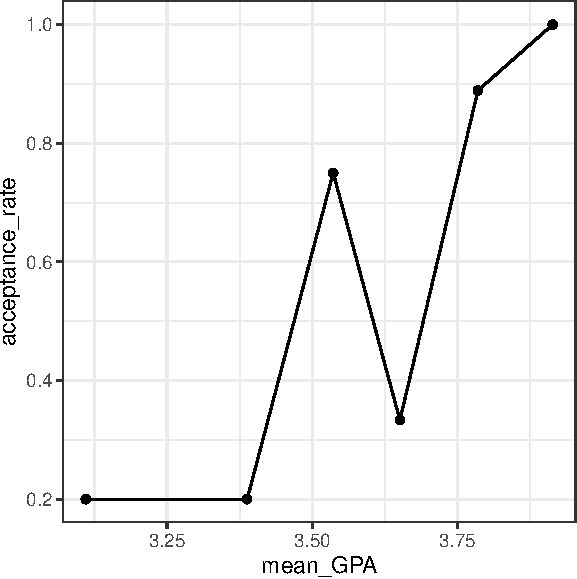
\includegraphics{MultLogSC_files/figure-latex/unnamed-chunk-52-1} \end{center}

\begin{itemize}
\tightlist
\item
  Augment the model \texttt{mod}. Create predictions on the scale of the
  response variable by using the \texttt{type.predict} argument.
\end{itemize}

\begin{Shaded}
\begin{Highlighting}[]
\CommentTok{# augmented model}
\NormalTok{MedGPA_plus <-}\StringTok{ }\NormalTok{mod }\OperatorTok
\StringTok{  }\KeywordTok{augment}\NormalTok{(}\DataTypeTok{type.predict =} \StringTok{"response"}\NormalTok{)}
\end{Highlighting}
\end{Shaded}

\begin{itemize}
\tightlist
\item
  Use \texttt{geom\_line()} to illustrate the model through the fitted
  values.
\end{itemize}

\begin{Shaded}
\begin{Highlighting}[]
\CommentTok{# logistic model on probability scale}
\NormalTok{data_space }\OperatorTok{+}
\StringTok{  }\KeywordTok{geom_line}\NormalTok{(}\DataTypeTok{data =}\NormalTok{ MedGPA_plus, }\KeywordTok{aes}\NormalTok{(}\DataTypeTok{x =}\NormalTok{ GPA, }\DataTypeTok{y =}\NormalTok{ .fitted), }\DataTypeTok{color =} \StringTok{"red"}\NormalTok{)}
\end{Highlighting}
\end{Shaded}

\begin{center}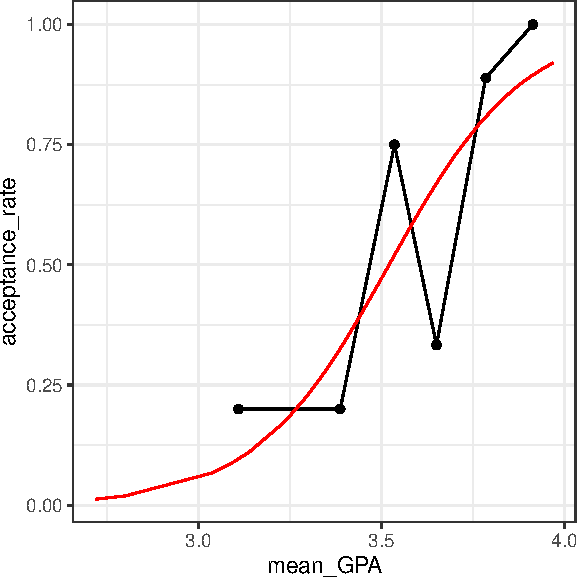
\includegraphics{MultLogSC_files/figure-latex/unnamed-chunk-54-1} \end{center}

The logistic predictions seem to follow the binned values pretty well.

\begin{center}\rule{0.5\linewidth}{\linethickness}\end{center}

\section{Odds scale}\label{odds-scale}

For most people, the idea that we could estimate the probability of
being admitted to medical school based on undergraduate GPA is fairly
intuitive. However, thinking about how the probability changes as a
function of GPA is complicated by the non-linear logistic curve. By
translating the response from the probability scale to the
\href{https://en.wikipedia.org/wiki/Odds}{odds} scale, we make the right
hand side of our equation easier to understand.

If the probability of getting accepted is \(y\), then the odds are
\(y/(1-y)\). Expressions of probabilities in terms of odds are common in
many situations, perhaps most notably gambling.

Here we are plotting \(y\)/(\(1-y\))as a function of \(x\), where that
function is

\begin{equation}
\text{odds}(\hat{y})=\frac{\hat{y}}{1 - \hat{y}}=\exp(\hat{\beta}_0 + \hat{\beta}_1 \cdot x)
\end{equation}

Note that the left hand side is the expected odds of being accepted to
medical school. The right hand side is now a familiar exponential
function of \(x\).

The \texttt{MedGPA\_binned} data frame contains the data for each GPA
bin, while the \texttt{MedGPA\_plus} data frame records the original
observations after being \texttt{augment()}-ed by \texttt{mod}.

\begin{center}\rule{0.5\linewidth}{\linethickness}\end{center}

\subsection*{Exercise}\label{exercise-17}
\addcontentsline{toc}{subsection}{Exercise}

\begin{itemize}
\tightlist
\item
  Add a variable called \texttt{odds} to \texttt{MedGPA\_binned} that
  records the odds of being accepted to medical school for each bin.
\end{itemize}

\begin{Shaded}
\begin{Highlighting}[]
\CommentTok{# compute odds for bins}
\NormalTok{MedGPA_binned <-}\StringTok{ }\NormalTok{MedGPA_binned }\OperatorTok
\StringTok{  }\KeywordTok{mutate}\NormalTok{(}\DataTypeTok{odds =}\NormalTok{ acceptance_rate }\OperatorTok{/}\StringTok{ }\NormalTok{(}\DecValTok{1} \OperatorTok{-}\StringTok{ }\NormalTok{acceptance_rate))}
\end{Highlighting}
\end{Shaded}

\begin{itemize}
\tightlist
\item
  Create a scatterplot called \texttt{data\_space} for \texttt{odds} as
  a function of \texttt{mean\_GPA} using the binned data in
  \texttt{MedGPA\_binned}. Connect the points with
  \texttt{geom\_line()}.
\end{itemize}

\begin{Shaded}
\begin{Highlighting}[]
\CommentTok{# plot binned odds}
\NormalTok{data_space <-}\StringTok{ }\KeywordTok{ggplot}\NormalTok{(}\DataTypeTok{data =}\NormalTok{ MedGPA_binned, }
                     \KeywordTok{aes}\NormalTok{(}\DataTypeTok{x =}\NormalTok{ mean_GPA, }\DataTypeTok{y =}\NormalTok{ odds)) }\OperatorTok{+}\StringTok{ }
\StringTok{  }\KeywordTok{geom_point}\NormalTok{() }\OperatorTok{+}\StringTok{ }
\StringTok{  }\KeywordTok{geom_line}\NormalTok{() }\OperatorTok{+}\StringTok{ }
\StringTok{  }\KeywordTok{theme_bw}\NormalTok{()}
\NormalTok{data_space}
\end{Highlighting}
\end{Shaded}

\begin{center}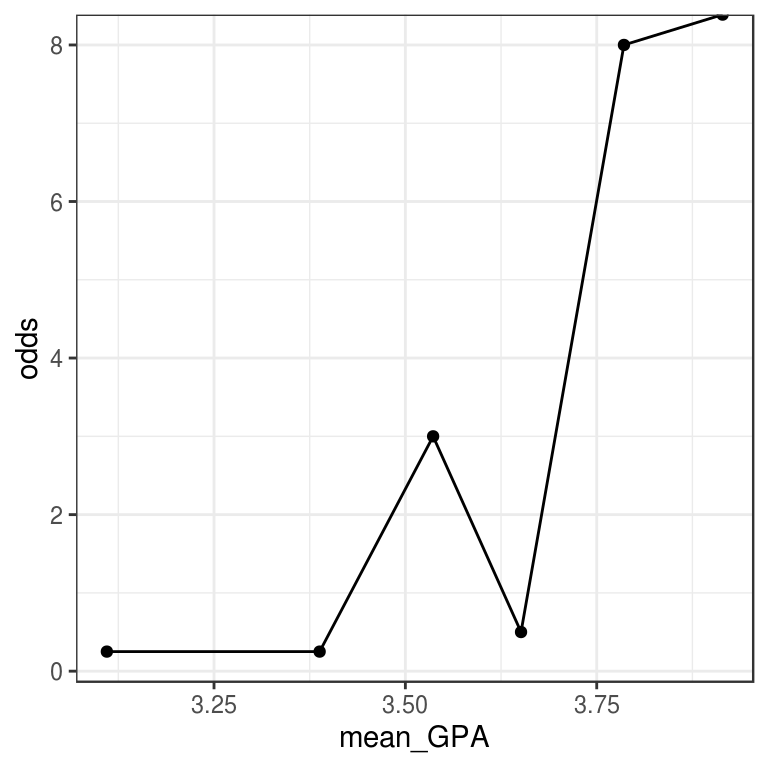
\includegraphics{MultLogSC_files/figure-latex/unnamed-chunk-56-1} \end{center}

\begin{itemize}
\tightlist
\item
  Add a variable called \texttt{odds\_hat} to \texttt{MedGPA\_plus} that
  records the predicted odds of being accepted for each observation.
\end{itemize}

\begin{Shaded}
\begin{Highlighting}[]
\CommentTok{# compute odds for observations}
\NormalTok{MedGPA_plus <-}\StringTok{ }\NormalTok{MedGPA_plus }\OperatorTok
\StringTok{  }\KeywordTok{mutate}\NormalTok{(}\DataTypeTok{odds_hat =}\NormalTok{ .fitted }\OperatorTok{/}\StringTok{ }\NormalTok{(}\DecValTok{1} \OperatorTok{-}\StringTok{ }\NormalTok{.fitted))}
\end{Highlighting}
\end{Shaded}

\begin{itemize}
\tightlist
\item
  Use \texttt{geom\_line()} to illustrate the model through the fitted
  values. Note that you should be plotting the \(\hat{odds}\)'s.
\end{itemize}

\begin{Shaded}
\begin{Highlighting}[]
\CommentTok{# logistic model on odds scale}
\NormalTok{data_space }\OperatorTok{+}
\StringTok{  }\KeywordTok{geom_line}\NormalTok{(}\DataTypeTok{data =}\NormalTok{ MedGPA_plus, }\KeywordTok{aes}\NormalTok{(}\DataTypeTok{x =}\NormalTok{ GPA, }\DataTypeTok{y =}\NormalTok{ odds_hat), }\DataTypeTok{color =} \StringTok{"red"}\NormalTok{)}
\end{Highlighting}
\end{Shaded}

\begin{center}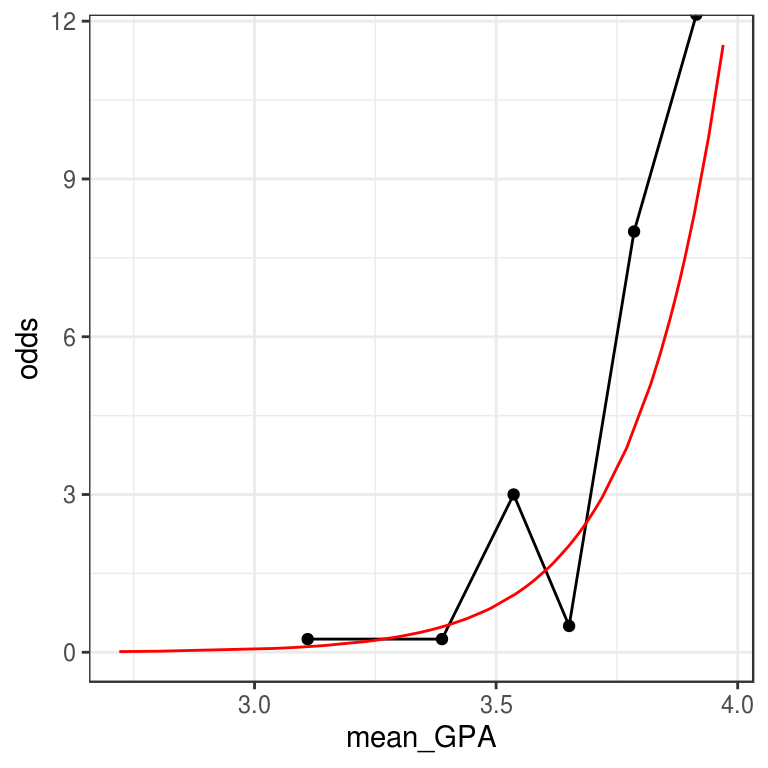
\includegraphics{MultLogSC_files/figure-latex/unnamed-chunk-58-1} \end{center}

\begin{center}\rule{0.5\linewidth}{\linethickness}\end{center}

\section{Log-odds scale}\label{log-odds-scale}

Previously, we considered two formulations of logistic regression
models:

\begin{itemize}
\item
  on the probability scale, the units are easy to interpret, but the
  function is non-linear, which makes it hard to understand
\item
  on the odds scale, the units are harder (but not impossible) to
  interpret, and the function is exponential, which makes it harder (but
  not impossible) to interpret
\end{itemize}

We'll now add a third formulation:

\begin{itemize}
\tightlist
\item
  on the log-odds scale, the units are nearly impossible to interpret,
  but the function is linear, which makes it easy to understand As you
  can see, none of these three is uniformly superior. Most people tend
  to interpret the fitted values on the probability scale and the
  function on the log-odds scale. The interpretation of the coefficients
  is most commonly done on the odds scale. Recall that we interpreted
  our slope coefficient \(\beta_1\) in linear regression as the expected
  change in \(y\) given a one unit change in \(x\). On the probability
  scale, the function is non-linear and so this approach won't work. On
  the log-odds, the function is linear, but the units are not
  interpretable (what does the log of the odds mean??). However, on the
  odds scale, a one unit change in \(x\) leads to the odds being
  multiplied by a factor of \(\hat{\beta_1}\). To see why, we form the
  odds ratio:
\end{itemize}

\begin{equation}
\text{OR}=\frac{\text{odds}(\hat{y}|x + 1)}{\text{odds}(\hat{y}|x)} = \exp \hat{\beta}_1
\end{equation}

Thus, the exponentiated coefficient \(\beta_1\) tells us how the
expected odds change for a one unit increase in the explanatory
variable. It is tempting to interpret this as a change in the expected
probability, but this is wrong and can lead to nonsensical predictions
(e.g.~expected probabilities greater than 1).

\begin{center}\rule{0.5\linewidth}{\linethickness}\end{center}

\subsection*{Exercise}\label{exercise-18}
\addcontentsline{toc}{subsection}{Exercise}

\begin{itemize}
\tightlist
\item
  Add a variable called \texttt{log\_odds} to \texttt{MedGPA\_binned}
  that records the odds of being accepted for each bin. Recall that
  \(odds(p) = p/(1-p)\).
\end{itemize}

\begin{Shaded}
\begin{Highlighting}[]
\CommentTok{# compute log odds for bins}
\NormalTok{MedGPA_binned <-}\StringTok{ }\NormalTok{MedGPA_binned }\OperatorTok
\StringTok{      }\KeywordTok{mutate}\NormalTok{(}\DataTypeTok{log_odds =} \KeywordTok{log}\NormalTok{(acceptance_rate }\OperatorTok{/}\StringTok{ }\NormalTok{(}\DecValTok{1} \OperatorTok{-}\StringTok{ }\NormalTok{acceptance_rate)))}
\end{Highlighting}
\end{Shaded}

\begin{itemize}
\tightlist
\item
  Create a scatterplot called \texttt{data\_space} for
  \texttt{log\_odds} as a function of \texttt{mean\_GPA} using the
  binned data in \texttt{MedGPA\_binned}. Use \texttt{geom\_line} to
  connect the points.
\end{itemize}

\begin{Shaded}
\begin{Highlighting}[]
\CommentTok{# plot binned log odds}
\NormalTok{data_space <-}\StringTok{ }\KeywordTok{ggplot}\NormalTok{(}\DataTypeTok{data =}\NormalTok{ MedGPA_binned, }
\KeywordTok{aes}\NormalTok{(}\DataTypeTok{y =}\NormalTok{ log_odds, }\DataTypeTok{x =}\NormalTok{ mean_GPA)) }\OperatorTok{+}\StringTok{ }
\StringTok{    }\KeywordTok{geom_point}\NormalTok{() }\OperatorTok{+}
\StringTok{    }\KeywordTok{geom_line}\NormalTok{() }\OperatorTok{+}\StringTok{ }
\StringTok{    }\KeywordTok{theme_bw}\NormalTok{()}
\NormalTok{data_space}
\end{Highlighting}
\end{Shaded}

\begin{center}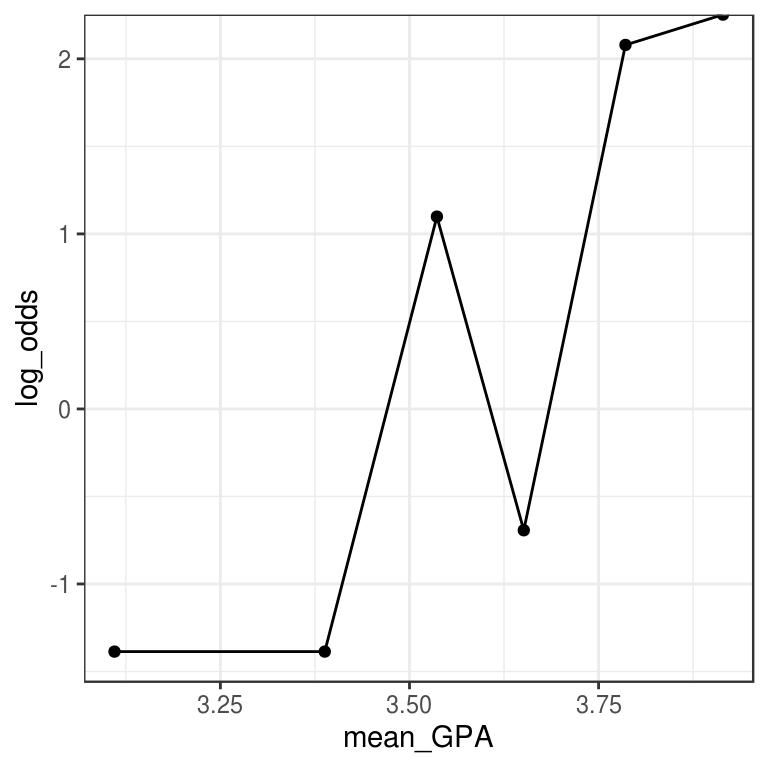
\includegraphics{MultLogSC_files/figure-latex/unnamed-chunk-60-1} \end{center}

\begin{itemize}
\tightlist
\item
  Add a variable called \texttt{log\_odds\_hat} to \texttt{MedGPA\_plus}
  that records the predicted odds of being accepted for each
  observation.
\end{itemize}

\begin{Shaded}
\begin{Highlighting}[]
\CommentTok{# compute log odds for observations}
\NormalTok{MedGPA_plus <-}\StringTok{ }\NormalTok{MedGPA_plus }\OperatorTok
\StringTok{  }\KeywordTok{mutate}\NormalTok{(}\DataTypeTok{log_odds_hat =} \KeywordTok{log}\NormalTok{(.fitted }\OperatorTok{/}\StringTok{ }\NormalTok{(}\DecValTok{1} \OperatorTok{-}\StringTok{ }\NormalTok{.fitted)))}
\end{Highlighting}
\end{Shaded}

\begin{itemize}
\tightlist
\item
  Use \texttt{geom\_line()} to illustrate the model through the fitted
  values. Note that you should be plotting the
  \(\widehat{\text{odds}}\)'s.
\end{itemize}

\begin{Shaded}
\begin{Highlighting}[]
\CommentTok{# logistic model on log odds scale}
\NormalTok{data_space }\OperatorTok{+}
\StringTok{  }\KeywordTok{geom_line}\NormalTok{(}\DataTypeTok{data =}\NormalTok{ MedGPA_plus, }\KeywordTok{aes}\NormalTok{(}\DataTypeTok{x =}\NormalTok{ GPA, }\DataTypeTok{y =}\NormalTok{ log_odds_hat), }\DataTypeTok{color =} \StringTok{"red"}\NormalTok{)}
\end{Highlighting}
\end{Shaded}

\begin{center}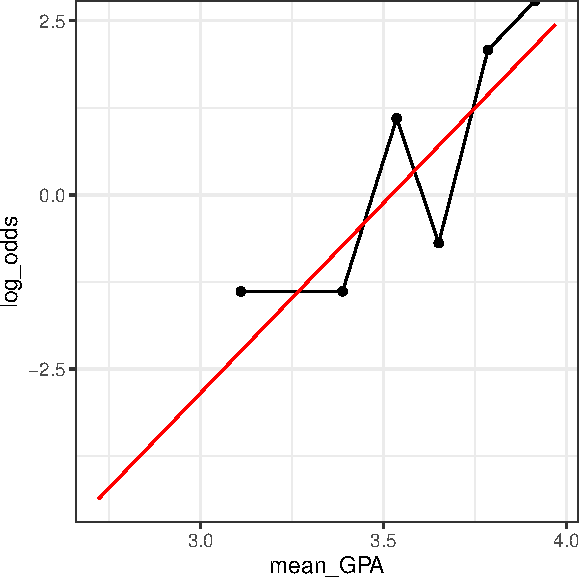
\includegraphics{MultLogSC_files/figure-latex/unnamed-chunk-62-1} \end{center}

When you're on the log-odds scale, your model is a simple linear
function.

\begin{center}\rule{0.5\linewidth}{\linethickness}\end{center}

\subsection*{Interpretation of logistic
regression}\label{interpretation-of-logistic-regression}
\addcontentsline{toc}{subsection}{Interpretation of logistic regression}

The fitted coefficient \(\hat\beta_1\) from the medical school logistic
regression model is 5.45. The exponential of this is 233.73.

Donald's GPA is 2.9, and thus the model predicts that the probability of
him getting into medical school is 3.26\%. The odds of Donald getting
into medical school are 0.0337, or---phrased in gambling terms---29.6:1.
If Donald hacks the school's registrar and changes his GPA to 3.9, then
which of the following statements is \textbf{FALSE}:

\begin{itemize}
\item
  His expected odds of getting into medical school improve to 7.8833 (or
  about 9:8).
\item
  His expected probability of getting into medical school improves to
  88.7\%.
\item
  His expected log-odds of getting into medical school improve by 5.45.
\item
  \textbf{His expected probability of getting into medical school
  improves to 7.9\%.} This is a FALSE statement.
\end{itemize}

\begin{center}\rule{0.5\linewidth}{\linethickness}\end{center}

\section{Making probabilistic
predictions}\label{making-probabilistic-predictions}

Just as we did with linear regression, we can use our logistic
regression model to make predictions about new observations. In this
exercise, we will use the \texttt{newdata} argument to the
\texttt{augment()} function from the \texttt{broom} package to make
predictions about students who were not in our original data set. These
predictions are sometimes called \emph{out-of-sample}.

Following our previous discussion about scales, with logistic regression
it is important that we specify on which scale we want the predicted
values. Although the default is \texttt{link} -- which uses the log-odds
scale -- we want our predictions on the probability scale, which is the
scale of the \texttt{response} variable. The \texttt{type.predict}
argument to \texttt{augment()} controls this behavior.

\begin{center}\rule{0.5\linewidth}{\linethickness}\end{center}

\subsection*{Exercise}\label{exercise-19}
\addcontentsline{toc}{subsection}{Exercise}

\begin{itemize}
\tightlist
\item
  Create a new data frame which has one variable called \texttt{GPA} and
  one row, with the value 3.51.
\end{itemize}

\begin{Shaded}
\begin{Highlighting}[]
\CommentTok{# create new data frame}
\NormalTok{new_data <-}\StringTok{ }\KeywordTok{data.frame}\NormalTok{(}\DataTypeTok{GPA =} \FloatTok{3.51}\NormalTok{)}
\end{Highlighting}
\end{Shaded}

\begin{itemize}
\tightlist
\item
  Use \texttt{augment()} to find the expected probability of admission
  to medical school for a student with a GPA of 3.51.
\end{itemize}

\begin{Shaded}
\begin{Highlighting}[]
\CommentTok{# make predictions}
\KeywordTok{augment}\NormalTok{(mod, }\DataTypeTok{newdata =}\NormalTok{ new_data, }\DataTypeTok{type.predict =} \StringTok{"response"}\NormalTok{)}
\end{Highlighting}
\end{Shaded}

\begin{verbatim}
# A tibble: 1 x 3
    GPA .fitted .se.fit
  <dbl>   <dbl>   <dbl>
1  3.51   0.484  0.0834
\end{verbatim}

By framing your prediction as a probability you can show how likely it
is that this student will get admitted to medical school.

\begin{center}\rule{0.5\linewidth}{\linethickness}\end{center}

\section{Making binary predictions}\label{making-binary-predictions}

Naturally, we want to know how well our model works. Did it predict
acceptance for the students who were actually accepted to medical
school? Did it predict rejections for the student who were not admitted?
These types of predictions are called in-sample. One common way to
evaluate models with a binary response is with a
\href{https://en.wikipedia.org/wiki/Confusion_matrix}{confusion matrix}.
{[}Yes, that is actually what it is called!{]}

However, note that while our response variable is binary, our fitted
values are probabilities. Thus, we have to round them somehow into
binary predictions. While the probabilities convey more information, we
might ultimately have to make a decision, and so this rounding is common
in practice. There are many different ways to round, but for simplicity
we will predict admission if the fitted probability is greater than 0.5,
and rejection otherwise.

First, we'll use \texttt{augment()} to make the predictions, and then
\texttt{mutate()} and \texttt{round()} to convert these probabilities
into binary decisions. Then we will form the confusion matrix using the
\texttt{table()} function. \texttt{table()} will compute a 2-way table
when given a data frame with two categorical variables, so we will first
use \texttt{select()} to grab only those variables.

You will find that this model made only 15 mistakes on these 55
observations, so it is nearly 73\% accurate.

\begin{center}\rule{0.5\linewidth}{\linethickness}\end{center}

\subsection*{Exercise}\label{exercise-20}
\addcontentsline{toc}{subsection}{Exercise}

The model object \texttt{mod} is already in your workspace.

\begin{itemize}
\tightlist
\item
  Create a data frame with the actual observations, and their fitted
  probabilities, and add a new column with the binary decision by
  rounding the fitted probabilities.
\end{itemize}

\begin{Shaded}
\begin{Highlighting}[]
\CommentTok{# data frame with binary predictions}
\NormalTok{tidy_mod <-}\StringTok{ }\KeywordTok{augment}\NormalTok{(mod, }\DataTypeTok{type.predict =} \StringTok{"response"}\NormalTok{) }\OperatorTok\StringTok{ }
\StringTok{  }\KeywordTok{mutate}\NormalTok{(}\DataTypeTok{Acceptance_hat =} \KeywordTok{round}\NormalTok{(.fitted)) }
\end{Highlighting}
\end{Shaded}

\begin{itemize}
\tightlist
\item
  Compute the confusion matrix between the actual and predicted
  acceptance.
\end{itemize}

\begin{Shaded}
\begin{Highlighting}[]
\CommentTok{# confusion matrix}
\NormalTok{tidy_mod }\OperatorTok\StringTok{ }
\StringTok{  }\KeywordTok{select}\NormalTok{(Acceptance, Acceptance_hat) }\OperatorTok
\StringTok{  }\KeywordTok{table}\NormalTok{()}
\end{Highlighting}
\end{Shaded}

\begin{verbatim}
          Acceptance_hat
Acceptance  0  1
         0 16  9
         1  6 24
\end{verbatim}

\chapter{Case Study: Italian restaurant in
NYC}\label{case-study-italian-restaurant-in-nyc}

Explore the relationship between price and the quality of food, service,
and decor for Italian restaurants in NYC.

\begin{center}\rule{0.5\linewidth}{\linethickness}\end{center}

\subsection*{Exploratory data analysis}\label{exploratory-data-analysis}
\addcontentsline{toc}{subsection}{Exploratory data analysis}

Multiple regression can be an effective technique for understanding how
a response variable changes as a result of changes to more than one
explanatory variable. But it is not magic -- understanding the
relationships among the explanatory variables is also necessary, and
will help us build a better model. This process is often called
\href{https://en.wikipedia.org/wiki/Exploratory_data_analysis}{exploratory
data analysis} (EDA) and is covered in another DataCamp course.

One quick technique for jump-starting EDA is to examine all of the
pairwise scatterplots in your data. This can be achieved using the
\texttt{pairs()} function. Look for variables in the \texttt{nyc} data
set that are strongly correlated, as those relationships will help us
check for
\href{https://en.wikipedia.org/wiki/Multicollinearity}{multicollinearity}
later on.

\begin{center}\rule{0.5\linewidth}{\linethickness}\end{center}

\subsection*{Excercise}\label{excercise}
\addcontentsline{toc}{subsection}{Excercise}

Which pairs of variables appear to be strongly correlated?

\begin{Shaded}
\begin{Highlighting}[]
\KeywordTok{pairs}\NormalTok{(nyc)}
\end{Highlighting}
\end{Shaded}

\begin{center}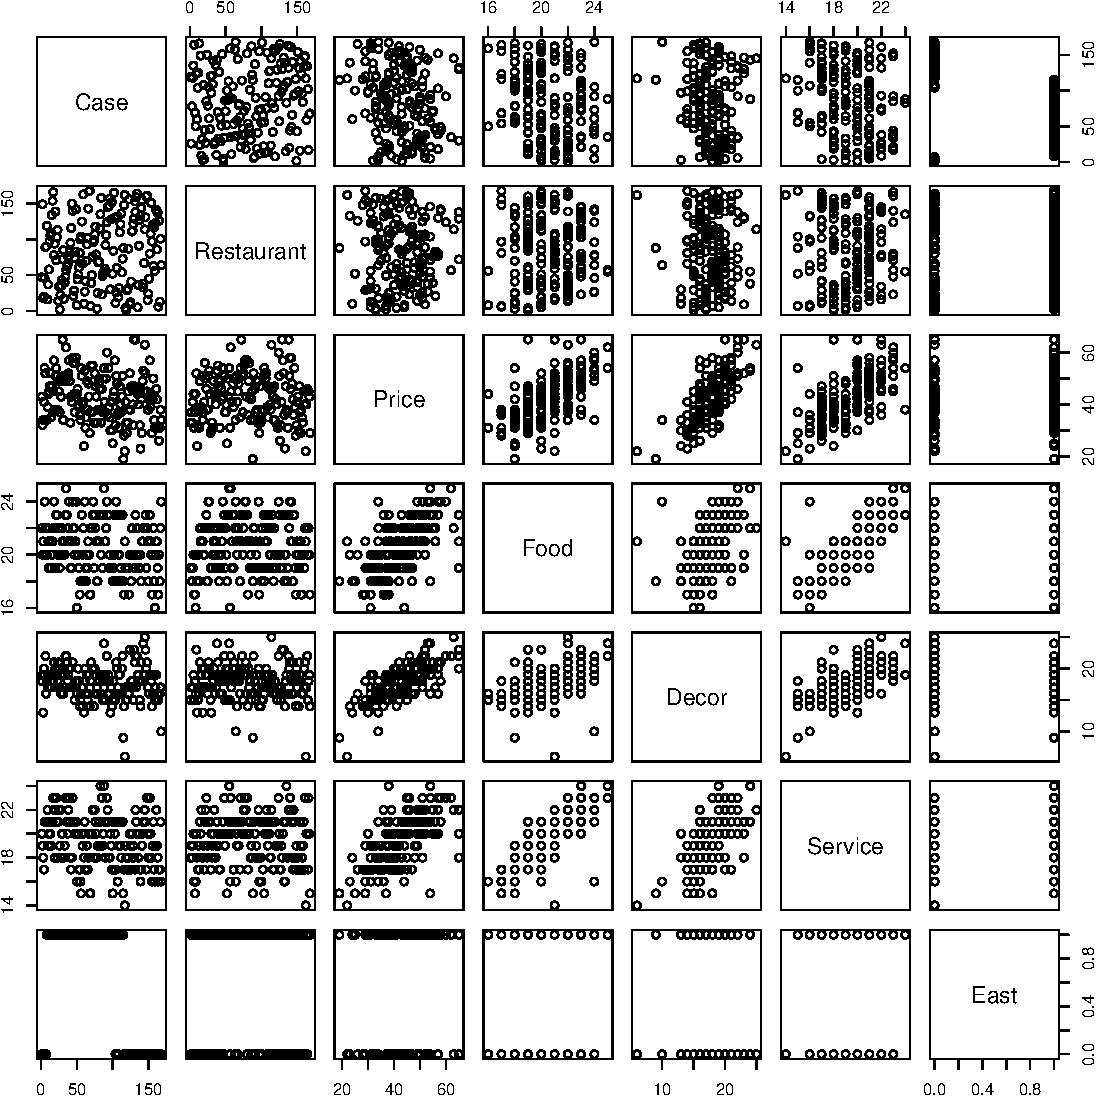
\includegraphics{MultLogSC_files/figure-latex/unnamed-chunk-68-1} \end{center}

\begin{itemize}
\item
  Case and Decor.
\item
  Restaurant and Price.
\item
  \textbf{Price and Food.}
\item
  Price and East.
\end{itemize}

\begin{center}\rule{0.5\linewidth}{\linethickness}\end{center}

\section{SLR models}\label{slr-models}

Based on your knowledge of the restaurant industry, do you think that
the quality of the food in a restaurant is an important determinant of
the price of a meal at that restaurant? It would be hard to imagine that
it wasn't. We'll start our modeling process by plotting and fitting a
model for \texttt{Price} as a function of \texttt{Food}.

On your own, interpret these coefficients and examine the fit of the
model. What does the coefficient of \texttt{Food} mean in plain English?
``Each additional rating point of food quality is associated with
a\ldots{}''

\begin{center}\rule{0.5\linewidth}{\linethickness}\end{center}

\subsection*{Exercise}\label{exercise-21}
\addcontentsline{toc}{subsection}{Exercise}

\begin{itemize}
\tightlist
\item
  Use \texttt{ggplot} to make a scatter plot for \texttt{Price} as a
  function of \texttt{Food}.
\end{itemize}

\begin{Shaded}
\begin{Highlighting}[]
\CommentTok{# Price by Food plot}
\KeywordTok{ggplot}\NormalTok{(}\DataTypeTok{data =}\NormalTok{ nyc, }\KeywordTok{aes}\NormalTok{(}\DataTypeTok{x =}\NormalTok{ Food, }\DataTypeTok{y =}\NormalTok{ Price)) }\OperatorTok{+}\StringTok{ }
\StringTok{  }\KeywordTok{geom_point}\NormalTok{() }\OperatorTok{+}\StringTok{ }
\StringTok{  }\KeywordTok{theme_bw}\NormalTok{()}
\end{Highlighting}
\end{Shaded}

\begin{center}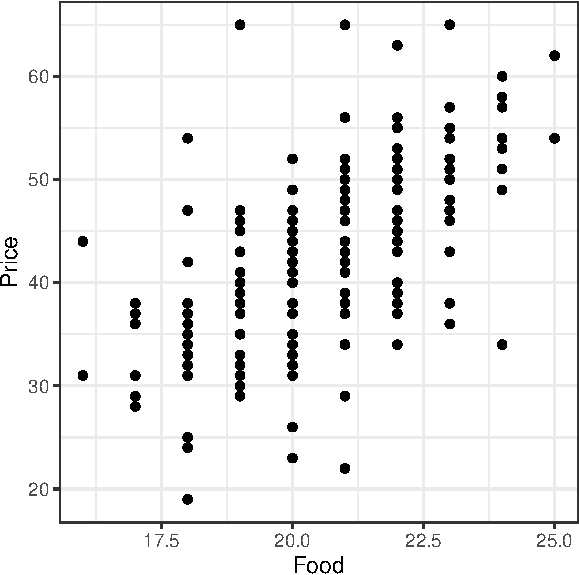
\includegraphics{MultLogSC_files/figure-latex/unnamed-chunk-69-1} \end{center}

\begin{itemize}
\tightlist
\item
  Use \texttt{lm()} to fit a simple linear regression model for
  \texttt{Price} as a function of \texttt{Food}.
\end{itemize}

\begin{Shaded}
\begin{Highlighting}[]
\CommentTok{# Price by Food model}
\KeywordTok{lm}\NormalTok{(Price }\OperatorTok{~}\StringTok{ }\NormalTok{Food, }\DataTypeTok{data =}\NormalTok{ nyc)}
\end{Highlighting}
\end{Shaded}

\begin{verbatim}

Call:
lm(formula = Price ~ Food, data = nyc)

Coefficients:
(Intercept)         Food  
    -17.832        2.939  
\end{verbatim}

What does the simple linear model say about how food quality affects
price?

\begin{center}\rule{0.5\linewidth}{\linethickness}\end{center}

\section{Parallel lines with
location}\label{parallel-lines-with-location}

In real estate, a common mantra is that the three most important factors
in determining the price of a property are ``location, location, and
location.'' If location drives up property values and rents, then we
might imagine that location would increase a restaurant's costs, which
would result in them having higher prices. In many parts of New York,
the east side (east of 5th Avenue) is more developed and perhaps more
expensive. {[}This is increasingly less true, but was more true at the
time these data were collected.{]}

Let's expand our model into a parallel slopes model by including the
East variable in addition to Food.

Use \texttt{lm()} to fit a parallel slopes model for \texttt{Price} as a
function of \texttt{Food} and \texttt{East}. Interpret the coefficients
and the fit of the model. Can you explain the meaning of the coefficient
on \texttt{East} in simple terms? Did the coefficient on \texttt{Food}
change from the previous model? If so, why? Did it change by a lot or
just a little?

Identify the statement that is \emph{FALSE}:

\begin{center}\rule{0.5\linewidth}{\linethickness}\end{center}

\begin{Shaded}
\begin{Highlighting}[]
\KeywordTok{lm}\NormalTok{(Price }\OperatorTok{~}\StringTok{ }\NormalTok{Food }\OperatorTok{+}\StringTok{ }\NormalTok{East, }\DataTypeTok{data =}\NormalTok{ nyc)}
\end{Highlighting}
\end{Shaded}

\begin{verbatim}

Call:
lm(formula = Price ~ Food + East, data = nyc)

Coefficients:
(Intercept)         Food         East  
    -17.430        2.875        1.459  
\end{verbatim}

\begin{itemize}
\item
  Each additional rating point of food quality is associated with a
  \$2.88 increase in the expected price of meal, after controlling for
  location.
\item
  The premium for an Italian restaurant in NYC associated with being on
  the east side of 5th Avenue is \$1.46, after controlling for the
  quality of the food.
\item
  \textbf{The change in the coefficient of food from \$2.94 in the
  simple linear model to \$2.88 in this model has profound practical
  implications for restaurant owners.}
\item
  None of the above.
\end{itemize}

\begin{center}\rule{0.5\linewidth}{\linethickness}\end{center}

\section{A plane in 3D}\label{a-plane-in-3d}

One reason that many people go to a restaurant---apart from the
food---is that they don't have to cook or clean up. Many people
appreciate the experience of being waited upon, and we can all agree
that the quality of the service at restaurants varies widely. Are people
willing to pay more for better restaurant \texttt{Service}? More
interestingly, are they willing to pay more for better service, after
controlling for the quality of the food?

Multiple regression gives us a way to reason about these questions. Fit
the model with \texttt{Food} and \texttt{Service} and interpret the
coefficients and fit. Did the coefficient on Food change from the
previous model? What do the coefficients on \texttt{Food} and
\texttt{Service} tell you about how these restaurants set prices?

Next, let's visually assess our model using \texttt{plotly}. The
\texttt{x} and \texttt{y} vectors, as well as the \texttt{plane} matrix,
have been created for you.

\begin{Shaded}
\begin{Highlighting}[]
\NormalTok{hmod <-}\StringTok{ }\KeywordTok{lm}\NormalTok{(Price }\OperatorTok{~}\StringTok{ }\NormalTok{Food }\OperatorTok{+}\StringTok{ }\NormalTok{Service, }\DataTypeTok{data =}\NormalTok{ nyc)}
\KeywordTok{summary}\NormalTok{(hmod)}\OperatorTok{$}\NormalTok{coef}
\end{Highlighting}
\end{Shaded}

\begin{verbatim}
              Estimate Std. Error   t value     Pr(>|t|)
(Intercept) -21.158582  5.6651431 -3.734872 2.583345e-04
Food          1.495369  0.4462060  3.351297 9.971979e-04
Service       1.704101  0.4184986  4.071939 7.220788e-05
\end{verbatim}

\begin{Shaded}
\begin{Highlighting}[]
\NormalTok{x <-}\StringTok{ }\KeywordTok{seq}\NormalTok{(}\DecValTok{16}\NormalTok{, }\DecValTok{25}\NormalTok{, }\DataTypeTok{length =} \DecValTok{50}\NormalTok{)}
\NormalTok{y <-}\StringTok{ }\KeywordTok{seq}\NormalTok{(}\DecValTok{14}\NormalTok{, }\DecValTok{24}\NormalTok{, }\DataTypeTok{length =} \DecValTok{50}\NormalTok{)}
\NormalTok{plane <-}\StringTok{ }\KeywordTok{outer}\NormalTok{(x, y, }\ControlFlowTok{function}\NormalTok{(a, b)\{}\OperatorTok{-}\FloatTok{21.158582} \OperatorTok{+}\StringTok{ }\FloatTok{1.495369}\OperatorTok{*}\NormalTok{a }\OperatorTok{+}\StringTok{ }\FloatTok{1.704101}\OperatorTok{*}\NormalTok{b\})}
\end{Highlighting}
\end{Shaded}

\begin{center}\rule{0.5\linewidth}{\linethickness}\end{center}

\subsection*{Exercise}\label{exercise-22}
\addcontentsline{toc}{subsection}{Exercise}

\begin{itemize}
\tightlist
\item
  Use \texttt{lm()} to fit a multiple regression model for
  \texttt{Price} as a function of \texttt{Food} and \texttt{Service}.
\end{itemize}

\begin{Shaded}
\begin{Highlighting}[]
\CommentTok{# fit model}
\KeywordTok{lm}\NormalTok{(Price }\OperatorTok{~}\StringTok{ }\NormalTok{Food }\OperatorTok{+}\StringTok{ }\NormalTok{Service, }\DataTypeTok{data =}\NormalTok{ nyc)}
\end{Highlighting}
\end{Shaded}

\begin{verbatim}

Call:
lm(formula = Price ~ Food + Service, data = nyc)

Coefficients:
(Intercept)         Food      Service  
    -21.159        1.495        1.704  
\end{verbatim}

\begin{itemize}
\tightlist
\item
  Use \texttt{plot\_ly} to draw 3D scatterplot for Price as a function
  of \texttt{Food} and \texttt{Service} by mapping the \texttt{z}
  variable to the response and the \texttt{x} and \texttt{y} variables
  to the explanatory variables. Place the food quality on the \(x\)-axis
  and service rating on the \(y\)-axis.
\end{itemize}

\begin{Shaded}
\begin{Highlighting}[]
\KeywordTok{library}\NormalTok{(plotly)}
\CommentTok{# draw 3D scatterplot}
\NormalTok{p <-}\StringTok{ }\KeywordTok{plot_ly}\NormalTok{(}\DataTypeTok{data =}\NormalTok{ nyc, }\DataTypeTok{z =} \OperatorTok{~}\StringTok{ }\NormalTok{Price, }\DataTypeTok{x =} \OperatorTok{~}\StringTok{ }\NormalTok{Food, }\DataTypeTok{y =} \OperatorTok{~}\StringTok{ }\NormalTok{Service, }\DataTypeTok{opacity =} \FloatTok{0.6}\NormalTok{) }\OperatorTok
\StringTok{  }\KeywordTok{add_markers}\NormalTok{() }
\NormalTok{p}
\end{Highlighting}
\end{Shaded}

\hypertarget{htmlwidget-3423e12707dfd0ca6570}{}

\begin{itemize}
\tightlist
\item
  Use \texttt{add\_surface()} to draw a plane through the cloud of
  points using the object \texttt{plane}.
\end{itemize}

\begin{Shaded}
\begin{Highlighting}[]
\CommentTok{# draw a plane}
\NormalTok{p }\OperatorTok
\StringTok{  }\KeywordTok{add_surface}\NormalTok{(}\DataTypeTok{x =} \OperatorTok{~}\NormalTok{x, }\DataTypeTok{y =} \OperatorTok{~}\NormalTok{y, }\DataTypeTok{z =} \OperatorTok{~}\StringTok{ }\NormalTok{plane, }\DataTypeTok{showscale =} \OtherTok{FALSE}\NormalTok{)}
\end{Highlighting}
\end{Shaded}

\hypertarget{htmlwidget-b38372eee96283519be5}{}

Is it surprising how service affects the price of a meal?

\begin{center}\rule{0.5\linewidth}{\linethickness}\end{center}

\section{Parallel planes with
location}\label{parallel-planes-with-location}

We have explored models that included the quality of both food and
service, as well as location, but we haven't put these variables all
into the same model. Let's now build a parallel planes model that
incorporates all three variables.

Examine the coefficients closely. Do they make sense based on what you
understand about these data so far? How did the coefficients change from
the previous models that you fit?

\begin{center}\rule{0.5\linewidth}{\linethickness}\end{center}

\subsection*{Exercise}\label{exercise-23}
\addcontentsline{toc}{subsection}{Exercise}

\begin{itemize}
\tightlist
\item
  Use \texttt{lm()} to fit a parallel planes model for \texttt{Price} as
  a function of \texttt{Food}, \texttt{Service}, and \texttt{East}.
\end{itemize}

\begin{Shaded}
\begin{Highlighting}[]
\CommentTok{# Price by Food and Service and East}
\KeywordTok{lm}\NormalTok{(Price }\OperatorTok{~}\StringTok{ }\NormalTok{Food }\OperatorTok{+}\StringTok{ }\NormalTok{Service }\OperatorTok{+}\StringTok{ }\NormalTok{East, }\DataTypeTok{data =}\NormalTok{ nyc)}
\end{Highlighting}
\end{Shaded}

\begin{verbatim}

Call:
lm(formula = Price ~ Food + Service + East, data = nyc)

Coefficients:
(Intercept)         Food      Service         East  
   -20.8155       1.4863       1.6647       0.9649  
\end{verbatim}

Does it seem like location has a big impact on price?

\begin{center}\rule{0.5\linewidth}{\linethickness}\end{center}

\subsection*{Interpretation of location
coefficient}\label{interpretation-of-location-coefficient}
\addcontentsline{toc}{subsection}{Interpretation of location
coefficient}

The fitted coefficients from the parallel planes model are listed below.

\begin{Shaded}
\begin{Highlighting}[]
\KeywordTok{lm}\NormalTok{(Price }\OperatorTok{~}\StringTok{ }\NormalTok{Food }\OperatorTok{+}\StringTok{ }\NormalTok{Service }\OperatorTok{+}\StringTok{ }\NormalTok{East, }\DataTypeTok{data =}\NormalTok{ nyc)}
\end{Highlighting}
\end{Shaded}

\begin{verbatim}

Call:
lm(formula = Price ~ Food + Service + East, data = nyc)

Coefficients:
(Intercept)         Food      Service         East  
   -20.8155       1.4863       1.6647       0.9649  
\end{verbatim}

Which of the following statements is \textbf{FALSE}?

Reason about the magnitude of the \texttt{East} coefficient.

\begin{center}\rule{0.5\linewidth}{\linethickness}\end{center}

\begin{itemize}
\item
  The premium for being on the East side of 5th Avenue is just less than
  a dollar, after controlling for the quality of food and service.
\item
  The impact of location is relatively small, since one additional
  rating point of either food or service would result in a higher
  expected price than moving a restaurant from the West side to the East
  side.
\item
  \textbf{The expected price of a meal on the East side is about 96\% of
  the cost of a meal on the West side, after controlling for the quality
  of food and service.}
\end{itemize}

\begin{center}\rule{0.5\linewidth}{\linethickness}\end{center}

\section{Impact of location}\label{impact-of-location}

The impact of location brings us to a modeling question: should we keep
this variable in our model? In a later course, you will learn how we can
conduct formal hypothesis tests to help us answer that question. In this
course, we will focus on the size of the effect. Is the impact of
location big or small?

One way to think about this would be in terms of the practical
significance. Is the value of the coefficient large enough to make a
difference to your average person? The units are in dollars so in this
case this question is not hard to grasp.

Another way is to examine the impact of location in the context of the
variability of the other variables. We can do this by building our
parallel planes in 3D and seeing how far apart they are. Are the planes
close together or far apart? Does the \texttt{East} variable clearly
separate the data into two distinct groups? Or are the points all mixed
up together?

\begin{Shaded}
\begin{Highlighting}[]
\NormalTok{modJ <-}\StringTok{ }\KeywordTok{lm}\NormalTok{(Price }\OperatorTok{~}\StringTok{ }\NormalTok{Food }\OperatorTok{+}\StringTok{ }\NormalTok{Service }\OperatorTok{+}\StringTok{ }\NormalTok{East, }\DataTypeTok{data =}\NormalTok{ nyc)}
\KeywordTok{summary}\NormalTok{(modJ)}\OperatorTok{$}\NormalTok{coef}
\end{Highlighting}
\end{Shaded}

\begin{verbatim}
               Estimate Std. Error    t value     Pr(>|t|)
(Intercept) -20.8154761  5.6843188 -3.6619121 0.0003373782
Food          1.4862725  0.4467122  3.3271368 0.0010831115
Service       1.6646884  0.4214169  3.9502175 0.0001157434
East          0.9648814  1.1363317  0.8491195 0.3970525764
\end{verbatim}

\begin{Shaded}
\begin{Highlighting}[]
\NormalTok{plane0 <-}\StringTok{ }\KeywordTok{outer}\NormalTok{(x, y, }\ControlFlowTok{function}\NormalTok{(a, b)\{}\OperatorTok{-}\FloatTok{20.8154761} \OperatorTok{+}\StringTok{ }\FloatTok{1.4862725}\OperatorTok{*}\NormalTok{a }\OperatorTok{+}\StringTok{ }\FloatTok{1.6646884}\OperatorTok{*}\NormalTok{b }\OperatorTok{+}\StringTok{ }\FloatTok{0.9648814}\NormalTok{\})}
\NormalTok{plane1 <-}\StringTok{ }\KeywordTok{outer}\NormalTok{(x, y, }\ControlFlowTok{function}\NormalTok{(a, b)\{}\OperatorTok{-}\FloatTok{20.8154761} \OperatorTok{+}\StringTok{ }\FloatTok{1.4862725}\OperatorTok{*}\NormalTok{a }\OperatorTok{+}\StringTok{ }\FloatTok{1.6646884}\OperatorTok{*}\NormalTok{b\})}
\end{Highlighting}
\end{Shaded}

\begin{center}\rule{0.5\linewidth}{\linethickness}\end{center}

\subsection*{Exercise}\label{exercise-24}
\addcontentsline{toc}{subsection}{Exercise}

\begin{itemize}
\tightlist
\item
  Use \texttt{plot\_ly} to draw 3D scatterplot for \texttt{Price} as a
  function of \texttt{Food}, \texttt{Service}, and \texttt{East} by
  mapping the \texttt{z} variable to the response and the \texttt{x} and
  \texttt{y} variables to the numeric explanatory variables. Use color
  to indicate the value of \texttt{East}. Place \texttt{Food} on the
  \(x\)-axis and \texttt{Service} on the \(y\)-axis.
\end{itemize}

\begin{Shaded}
\begin{Highlighting}[]
\KeywordTok{library}\NormalTok{(plotly)}
\CommentTok{# draw 3D scatterplot}
\NormalTok{p <-}\StringTok{ }\KeywordTok{plot_ly}\NormalTok{(}\DataTypeTok{data =}\NormalTok{ nyc, }\DataTypeTok{z =} \OperatorTok{~}\NormalTok{Price, }\DataTypeTok{x =} \OperatorTok{~}\NormalTok{Food, }\DataTypeTok{y =} \OperatorTok{~}\NormalTok{Service, }\DataTypeTok{opacity =} \FloatTok{0.6}\NormalTok{) }\OperatorTok
\StringTok{  }\KeywordTok{add_markers}\NormalTok{(}\DataTypeTok{color =} \OperatorTok{~}\KeywordTok{factor}\NormalTok{(East)) }
\NormalTok{p}
\end{Highlighting}
\end{Shaded}

\hypertarget{htmlwidget-9a853aba44393acce257}{}

\begin{itemize}
\tightlist
\item
  Use \texttt{add\_surface()} (twice) to draw two planes through the
  cloud of points, one for restaurants on the West side and another for
  restaurants on the East side. Use the objects \texttt{plane0} and
  \texttt{plane1}.
\end{itemize}

\begin{Shaded}
\begin{Highlighting}[]
\CommentTok{# draw two planes}
\NormalTok{p }\OperatorTok
\StringTok{  }\KeywordTok{add_surface}\NormalTok{(}\DataTypeTok{x =} \OperatorTok{~}\NormalTok{x, }\DataTypeTok{y =} \OperatorTok{~}\NormalTok{y, }\DataTypeTok{z =} \OperatorTok{~}\NormalTok{plane0, }\DataTypeTok{showscale =} \OtherTok{FALSE}\NormalTok{) }\OperatorTok
\StringTok{  }\KeywordTok{add_surface}\NormalTok{(}\DataTypeTok{x =} \OperatorTok{~}\NormalTok{x, }\DataTypeTok{y =} \OperatorTok{~}\NormalTok{y, }\DataTypeTok{z =} \OperatorTok{~}\NormalTok{plane1, }\DataTypeTok{showscale =} \OtherTok{FALSE}\NormalTok{)}
\end{Highlighting}
\end{Shaded}

\hypertarget{htmlwidget-03bd35ff25d219ccbead}{}

How does this visualization relate to the model coefficients you found
in the last exercise?

\begin{center}\rule{0.5\linewidth}{\linethickness}\end{center}

\section{Full model}\label{full-model}

One variable we haven't considered is \texttt{Decor}. Do people, on
average, pay more for a meal in a restaurant with nicer decor? If so,
does it still matter after controlling for the quality of food, service,
and location?

By adding a third numeric explanatory variable to our model, we lose the
ability to visualize the model in even three dimensions. Our model is
now a hyperplane -- or rather, parallel hyperplanes -- and while we
won't go any further with the geometry, know that we can continue to add
as many variables to our model as we want. As humans, our spatial
visualization ability taps out after three numeric variables (maybe you
could argue for four, but certainly no further), but neither the
mathematical equation for the regression model, nor the formula
specification for the model in R, is bothered by the higher
dimensionality.

Use \texttt{lm()} to fit a parallel planes model for \texttt{Price} as a
function of \texttt{Food}, \texttt{Service}, \texttt{Decor}, and
\texttt{East}.

\begin{Shaded}
\begin{Highlighting}[]
\KeywordTok{lm}\NormalTok{(Price }\OperatorTok{~}\StringTok{ }\NormalTok{Food }\OperatorTok{+}\StringTok{ }\NormalTok{Service }\OperatorTok{+}\StringTok{ }\NormalTok{Decor }\OperatorTok{+}\StringTok{ }\NormalTok{East, }\DataTypeTok{data =}\NormalTok{ nyc)}
\end{Highlighting}
\end{Shaded}

\begin{verbatim}

Call:
lm(formula = Price ~ Food + Service + Decor + East, data = nyc)

Coefficients:
(Intercept)         Food      Service        Decor         East  
 -24.023800     1.538120    -0.002727     1.910087     2.068050  
\end{verbatim}

Notice the dramatic change in the value of the \texttt{Service}
coefficient.

Which of the following interpretations is invalid?

\begin{center}\rule{0.5\linewidth}{\linethickness}\end{center}

\begin{itemize}
\item
  Since the quality of food, decor, and service were all strongly
  correlated, multicollinearity is the likely explanation.
\item
  Once we control for the quality of food, decor, and location, the
  additional information conveyed by service is negligible.
\item
  \textbf{Service is not an important factor in determining the price of
  a meal.} This is false!
\item
  None of the above.
\end{itemize}

\begin{center}\rule{0.5\linewidth}{\linethickness}\end{center}

\bibliography{book.bib,packages.bib}


\end{document}
